\documentclass[twocolumn]{article}
% \usepackage[english]{babel}
% \usepackage[T1]{fontenc}
% \usepackage{graphicx}
\usepackage{kpfonts}[maths]
\usepackage{libertine}
% \usepackage{placeins}
% \usepackage{gensymb}
\usepackage{fontspec}
\setmonofont[Mapping=tex-text]{inconsolata}
% \usepackage{subcaption}
% \usepackage{mdframed}
% \usepackage{caption}
\usepackage{amsmath}
% \usepackage{lipsum}
\usepackage{tikz}
% \usepackage{minted}
% \usepackage{lipsum}
% \usepackage{xcolor}
% \usepackage{sectsty}
\usepackage{hyperref}
% \usepackage{csquotes}
\usepackage[style=authoryear]{biblatex}
\usepackage[inline]{enumitem}


\newlist{inline-enum}{enumerate*}{1}
\setlist[inline-enum]{label=(\roman*)}

\hypersetup{
    colorlinks=true,
    urlcolor=blue,
    linkcolor=black,
    citecolor=black,
    breaklinks=true,
}

\definecolor{CERNblue}{HTML}{22529e}
\definecolor{CodeBg}{rgb}{0.95, 0.95, 0.95}

% \setminted{
%     % linenos=true,
%     autogobble=true,
%     frame=single,
%     % framesep=2mm,
%     % framerule=0.4pt,
%     tabsize=4,
%     fontsize=\footnotesize,
%     breaklines,
%     bgcolor=CodeBg,
% }

\usetikzlibrary{automata, positioning, arrows, shapes, calc}
\tikzset{
  ->, % make edges directed
  >=stealth, % make the arrow heads bold
  node distance=5.5cm, % minimum distance
  every state/.style={thick, fill=gray!10, ellipse}, % properties of state nodes
  initial text=Start, % text that aappears on the start arrow
  every text node part/.style={align=center}, % allow multiline node descriptions
}

\setlist[enumerate]{itemsep=0mm}
\setlist[itemize]{itemsep=-0mm}


% \sectionfont{\color{CERNblue}}
% \subsectionfont{\color{CERNblue}}
% \subsubsectionfont{\color{CERNblue}}

\newcommand{\hypermail}[1]{\href{mailto:#1}{\texttt{<#1>}}}

\addbibresource{ref.bib}

% TODO: add a link to the repository somewhere

\title{
D7039E/E7032E\footnote{Codes of courses taken by team members at Luleå Technical University.}
--- Project: Model, Simulation and Implementation of a Mechatronical System for Use in a Mimicked Industrial Environment
}
\author{
As authored/researched/developed by:\footnote{In no particular order; All team members can be contacted via \href{mailto:vikson-6@student.ltu.se;lukkar-4@student.ltu.se;sansim-6@student.ltu.se;olemis-6@student.ltu.se;rubasp-6@student.ltu.se;alinou-6@student.ltu.se;alikhar-6@student.ltu.se}{this hyperlink}.} \\
Viktor Sonesten \hypermail{vikson-6@student.ltu.se} \\
Lukas Karlsson \hypermail{lukkar-4@student.ltu.se} \\
Simon Sandberg \hypermail{sansim-6@student.ltu.se} \\
Oleksiy Mishchenko \hypermail{olemis-6@student.ltu.se} \\
Ruben Asplund \hypermail{rubasp-6@student.ltu.se} \\
Ali Nouri \hypermail{alinou-6@student.ltu.se} \\
Ali Khademi \hypermail{alikha-6@student.ltu.se}
}
\date{\today}                   % TODO: use latest date as reported by git

\begin{document}
\maketitle

\section{Introduction}
\subsection{Background}
% Introduce ARTEMIS and the Arrowhead project
The ARTEMIS\footnote{\textbf{A}dvanced \textbf{R}esearch \& \textbf{T}echnology for \textbf{EM}bedded \textbf{I}ntelligent \textbf{S}ystems} Industry Association is an organisation with the goal of innovating the embedded intelligent systems sector in Europe.~\parencite{artemis}
One of the approaches to reach this goal was the 2013 start of the ARROWHEAD project which ``[address] the efficiency and flexibility at the global scale by means of collaborative automation for five application verticals; [one of which being] production (manufacturing, process, energy).''~\parencite{arrowhead-project-call}

% Summarize the result of the project
The project concluded 2017 and yielded the Arrowhead Framework which enable interoperability between Internet of Things (IoT) devices by providing guarantees for:
\begin{inline-enum}
    \item real-time data handling;
    \item data and system security;
    \item automation system engineering; and
    \item scalability of automation systems.
\end{inline-enum}
\parencite{arrowhead-project-about}
With the above guarantees provided by Arrowhead, resources otherwise required for developing a new framework (ad-hoc or not) may instead be allotted to the system the framework ultimately will interact with.

% Describe the reason for this project.
% TODO: extend/rewrite; describe that the process of moving an object from a to b by use of robots have not been solved yet (mentioned during the second lecture).
The reason for this project is then to verify that Arrowhead can indeed be used to resolve a common industry problem: production; specifically the act of moving a object from one station to another,
which is a common procedure in product pipelines.

% TODO: mention that Arrowhead aims to create de-facto standards for European industrialization efforts?

% XXX: Currently disjointed from the background section: background has large focus on Arrowhead. This section does not.
\subsection{Problem description}
% Summarize the problem and describe that we're simulating a factory settings.
The problem this project aims to solve is that of automatically moving an object from a designated pick-up point to a designated drop-off point on a system-external signal.
In practise, the problem space aims to mimic the environment of a factory floor where an object under manufacture has been fully processed in a station and should be moved to the next.

% Boil the issue down to simple mathematical terms.
Described in different terms, the problem is the automatic displacement of an object from a origin point $(x_0, y_0, z_0)$ to a destination point $(x, y, z)$,
where $(x, y)$ denote a position on the factory floor and $y, y \geq 0$, an elevation above the floor.

% Mention the inclusion of Arrowhead in the problem.
Additionally, a station signals a fully processed object via the Arrowhead Framework in a local cloud.
Upon this signal, the task of moving the object is to be delegated to the system this project aims to develop.

% TODO: insert an image of the conveyor belt with measures.

\subsection{Limitations}
% Note and expound on the very large problem domain.
The problem domain is vast and infinite configurations can mimic the wanted factory setting:
\begin{inline-enum}
    \item different placement/rotations of one or more stations;
    \item obstacles of multiple types; static and dynamic (e.g. humans, other robots);
    \item recovery/discard of a dropped object; and
    \item conditional and/or time-dependent origin/destination points.
\end{inline-enum}
Support for more configurations require a more complex system design, simulation and implementation;
and more complexity requires more development time.

% Note time limitation and the smaller problem space we aim to tackle.
The system developed in this project is to be thoroughly modelled, simulated, and implemented in the time span of twelve weeks (weeks 36--48).
For that reason (and those stated in the previous paragraph), this project is thus limited to two stations:
a single designated pick-up point and a single designated drop-off point  --- both static and elevated (however, $z_0 = z$).
Furthermore, the system environment will contain no other obstacles, and if an object is dropped, the displacement procedure ends and is considered to have failed;
this project aims to implement a proof-of-concept solution for the stated problem, not a readily available product ready for industry integration.
If an object is successfully displaced automatically to its destination once, the project is considered a success.

% Note that the system has no real-time requirement
% XXX: unless we require the system to not overshoot its 2D destionations, then we need to process location data with known delay.
% TODO: find a reference on this statement.
Because the above defined problem domain lacks any time component (as would be the case if the system would need to dodge moving obstacles, respond to time-dependent destinations, etc.)
and because the object need only be moved to its destination eventually (as this is only a proof of concept), the implementation is under no real-time requirement.
This greatly lessens the requirement of the system model and software implementation.

\section{System design and composition}
\subsection{Model}
The system is modeled in two parts: the moving base and the\ldots
% TODO: describe the moving base, and the attachment, whatever it ends up being.
% Include physical models.


% Describe the states of the system.
We argue for the following five states of the system:
\begin{inline-enum}
\item waiting for a command;
\item moving to a destination;
\item following a navigation-line;
\item picking an object up; and
\item dropping an object off.
\end{inline-enum}
The relation between these five states are visually described in the state machine of Fig~\ref{fig:state_machine}.
\begin{figure*}[ht]
  \centering
  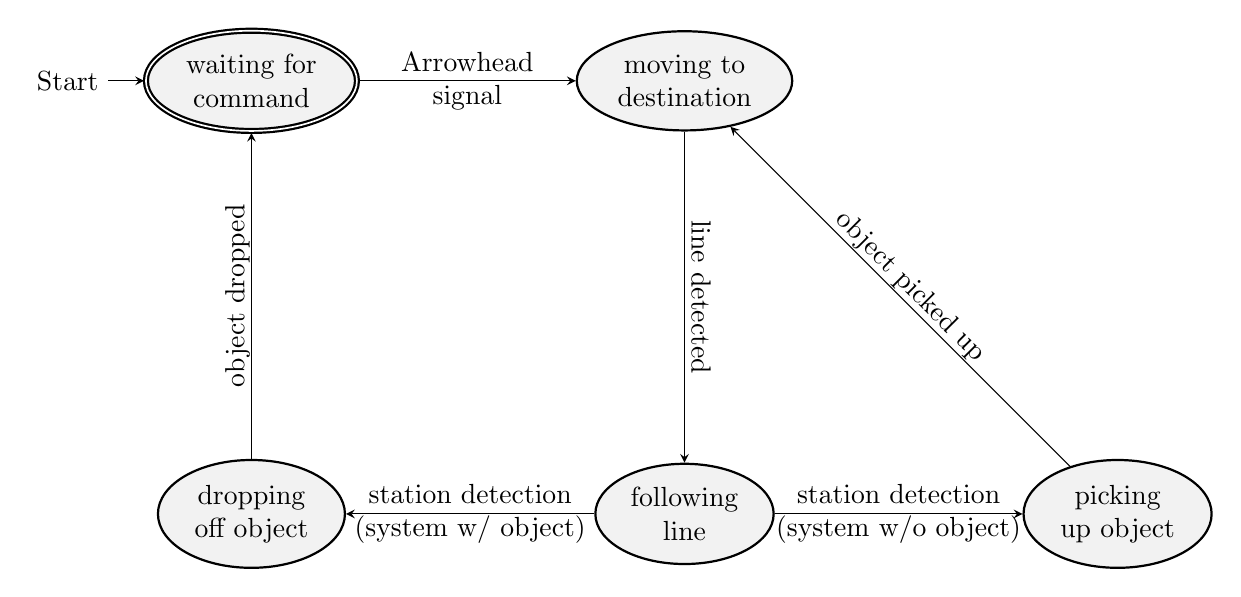
\begin{tikzpicture}
    \node[state, initial, accepting] (wait) {waiting for \\ command};
    \node[state, right of=wait] (move) {moving to \\ destination};
    \node[state, below of=move] (follow) {following \\ line};
    \node[state, right of=follow] (pickup) {picking \\ up object};
    \node[state, left of=follow] (dropoff) {dropping \\ off object};

    \path[->] (wait) edge node{Arrowhead \\ signal} (move)
    (move) edge[sloped] node{line detected \\} (follow)
    (follow) edge[sloped] node{station detection \\ (system w/o object)} (pickup)
    (follow) edge[sloped] node{station detection \\ (system w/ object)} (dropoff)
    (pickup) edge[sloped] node{object picked up \\} (move)
    (dropoff) edge[sloped] node{object dropped \\} (wait)
    ;
  \end{tikzpicture}
  \caption{High-level state machine of the system.}
  \label{fig:state_machine}
\end{figure*}
\subsubsection{Mobile platform}
\label{subsubsec:unicycle}
The model used in this case is the unicycle model, due to the differential steering. 
This is because of the mobile platform has only two wheels/trucks and it is not able to apply any steering angle to its wheels. 
The only way this robot can change orientation is by giving different velocity on each wheel-driving servo on left- and right- side. 
With this feature it is also possible to change the orientation of the mobile platform without changing the position of the platform. 
I.e. the robot is able to spin while the right-hand sidewheels have the same velocity as the left-hand side wheels, in opposite direction.\\ 
\begin{figure}[h!]
\centering
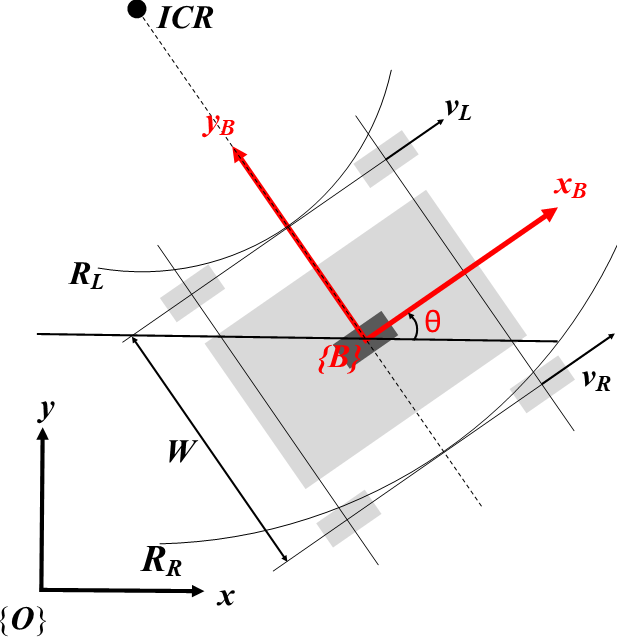
\includegraphics[width=0.4\textwidth]{sections/assets/car-unicycle.png}
\caption{Unicycle model of a car-like robot. 
$v_L$ and $v_R$ represent the left- and right-hand side wheels' velocities respectively. 
The robot follows a path around the instantaneous center of rotation (ICR) where $R_L$ and $R_R$ are the distances from left and right wheels to ICR respectively and $w$ is the distance between them.}
\label{fig:UnicycleModel}
\end{figure} 

As shown in Fig.~\ref{fig:UnicycleModel} The robot follows a curved path with the instantaneous center of rotation at its center. 
The left-hand side wheels have velocity $v_L$ and moves along an arc with radius $R_L$ during the time that right-hand side wheels moves along another arc with radius $R_R$ at the speed of $v_R$. 
The turning rate of the body is
\begin{equation*}
\dot{\theta}= \frac{v_L}{R_L} = \frac{v_R}{R_R}
\end{equation*}

since $R_R = R_L + W$ the expression can be simplified as
\begin{equation}
\dot{\theta}= \frac{v_R - v_L}{W} = \frac{v_\Delta}{W}\label{eq:ThetaDot}
\end{equation}

the equations of motion for this model are
\begin{eqnarray}
\begin{aligned}
\dot{x} &= v\,cos(\theta)\\
\dot{y} &= v\,sin(\theta)\\
\dot{\theta} &= \omega = \frac{v_\Delta}{W}
\end{aligned}
\label{eq:MotionEq}
\end{eqnarray}

where the average velocity\parencite{Corke2011} is given by        
\begin{equation}
v = \frac{v_R + v_L}{2} 
\label{eq:av_velocity}
\end{equation}

\subsection{Simulation}
% Simulte the models from the previous section and show that it will work.
% Motivate regulation approach.
\subsubsection{Mobile platform}
A simulation profile is made to make sure of the unicycle mode in sub section \ref{subsubsec:unicycle} is the suitable model for this application.
The simulation is made in discrete time domain with the sampling frequency of $10Hz$.
This is done in the described way due to the robot is going to operate in discrete time.
The sampling frequency is assumed to be low and that is because the designed controllers are going to be able to work fine for higher samplings frequencies but that is not guaranteed for vise-versa.\\  
As the unicycle model describes the systems dynamics.
The position of the robot $(x, y, \theta)$ is dependent on the two wheel velocities. Which in turn has dependencies to the average velocity $V$ and the angular velocity $\omega$. These relations are presented in Eq.(\ref{eq:ThetaDot}) - Eq.(\ref{eq:av_velocity}).\\
\begin{figure*}[ht]
\centering
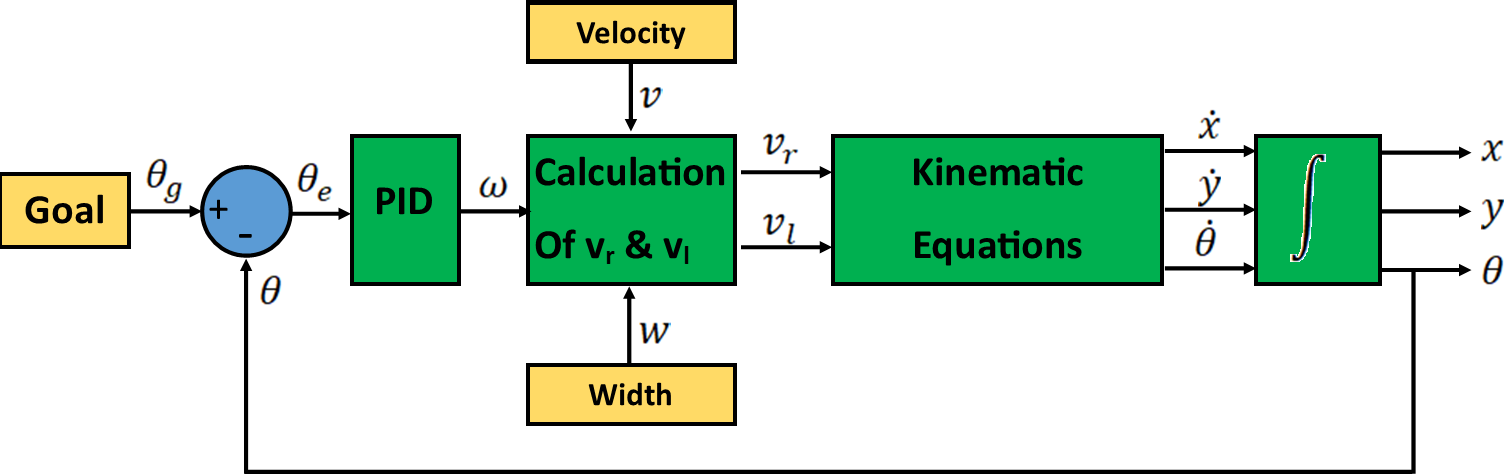
\includegraphics[width=\textwidth]{sections/assets/omegaCtrlr.png}
\caption{Overview of the systems block diagram where the angular velocity $\omega$ is controlled by a PID controller.}
\label{fig:overview}
\end{figure*} 

A pole placement analyze is required for the design of a PID controller.
This analyze is done in continues time domain, due to its simplicity.\\
As mentioned in Eq.(\ref{eq:MotionEq})
\begin{equation}
\dot{\theta} = \omega
\label{eq:omega}
\end{equation}

By taking the Laplace transform of Eq.(\ref{eq:omega}) gives:
\begin{equation}
s\cdot \Theta(s)= \Omega(s)
\end{equation}

Where $G(s)$ is the transfer function
\begin{equation}
\therefore G(s)=\frac{\Omega(s)}{s\cdot\Theta(s)} = 1
\end{equation}

However it is the angular position $\theta$ which is relevant in this case.
So it is required to implement an integrator in the feedback to make the angular position controllable.\\ \\
\tikzset{
    block/.style = {draw, rectangle, 
    minimum height=1cm, 
    minimum width=2cm},
    input/.style = {coordinate,node distance=1cm},
    output/.style = {coordinate,node distance=2cm},
    arrow/.style={draw, -latex,node distance=2cm},
    pinstyle/.style = {pin edge={latex-, black,node distance=2cm}},
    sum/.style = {draw, circle, node distance=1cm}
}
\begin{figure}[h]
    \begin{center}
        \begin{tikzpicture}[auto, node distance=2.5cm,>=latex']
        \node [input, name=input] {};
        \node [sum, right of=input] (sum) {};
        \node [block, right of=sum] (controller) {$PID$};
        \node [block, right of=controller] (plant) {$G(s)$};
        \node [output, right of=plant] (output) {};
        \node [block, below of=plant] (feedback) {$\frac{1}{s}$};
        \draw [draw,->] (input) -- node {$U(s)$} (sum);
        \draw [->] (sum) -- node {} (controller);
        \draw [->] (controller) -- node {} (plant);
        \draw [->] (plant) -- node [name=y] {$Y(s)$}(output);
        \draw [->] (y) |- node [above,pos=0.79] {} (feedback) ;
        \draw [->] (feedback) -| node[pos=0.99] {$-$} 
        node [near end] {} (sum);
        \end{tikzpicture}
    \end{center}
    \caption{Closed Loop system with a integrator in the feedback.}\label{fig:closedloop}
\end{figure}

In this case the closed loop transfer function will be as shown in Eq.(\ref{eq:closedloop})
\begin{equation}
G_{c}(s) = \frac{PID}{s + PID}
\label{eq:closedloop}
\end{equation} 

As the closed loop transfer function of the system is describing a first order system, it is possible to use a P-controller. 
I.e. the controller only has a proportional gain and doesn't require a integrative or derivative elements. 
So the final closed loop transfer function will be 
\begin{equation}
G_{c}(s) = \frac{K_p}{s + K_p}
\label{eq:kp}
\end{equation}

This system will have a pole at $-K_p$.
Any positive proportional gain will results in a stable pole and which in turn a stable system. \\
\begin{figure*}[ht]
\centering
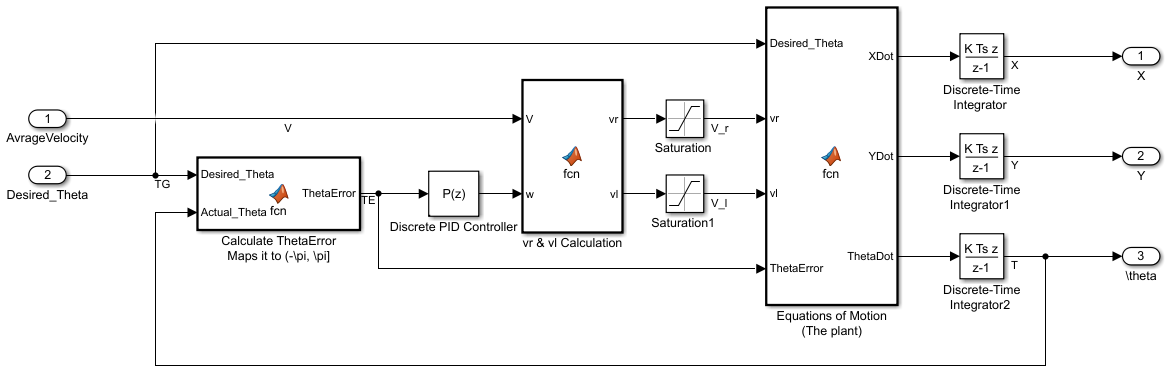
\includegraphics[width=\textwidth]{sections/assets/Theta_PID.PNG}
\caption{The complete control block for the angular position in discrete time domain.}
\label{fig:PID1}
\end{figure*}
\\
 
It is required to make sure that $\theta$ error, $\theta_e$ is in $(-\pi,\pi]$ span. Due to the $\theta = \theta \pm 2 \cdot n \cdot \pi$, it is possible for the error be in out of this span.
By using a function called arctan2 or atan2 in many programming languages it is possible to accomplish this challenge.\\
This function often has two input argument (y,x).\\ 
By defining 
\begin{equation}
\theta = atan2(sin(\theta),\, cos(\theta))
\end{equation}
$\theta$ will always be in $(-\pi,\pi]$ span.\\

Due to the physical limits the servos have, two saturation blocks are required.
These blocks are shown in figure(\ref{fig:PID1}) and the assumption for their limits are (-10,10) $[cm/sec]$. 
This assumption is done to make the simulation more alike the real application.\\
\begin{figure}[ht]
\centering
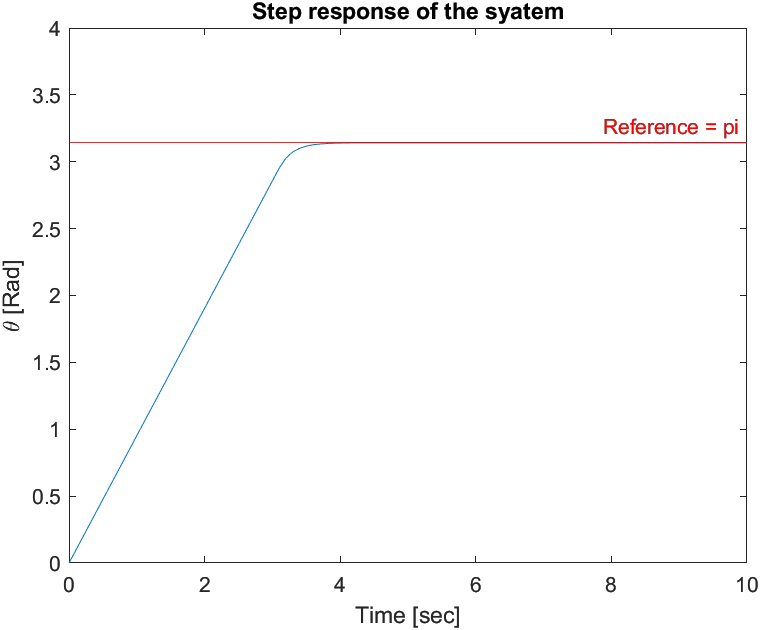
\includegraphics[width=0.4\textwidth]{sections/assets/Theta_pi_stepresponce.png}
\caption{The step response for $\theta$ where the proportional gain $K_p = 4$ and the reference value is $\pi$ .}
\label{fig:Theta_Step}
\end{figure}

The result of the simulation, the step response for the angular position control system is presented in figure(\ref{fig:Theta_Step}).
As it shown this is a stable system, it has no steady state error, no oscillation and relative fast rise-time.\\

In this part of the mobile platforms movement it is important to be able to control the spacial position $(x, y)$. 
As shown in the kinematic equations Eq.(\ref{eq:MotionEq}) the positions are dependent on both the angular velocity $\omega$ and the average velocity $v$. 
A design of a controller for the average velocity is required to make it possible to control the spacial position. 
Take note of the two input $AverageVelocity$, $Desired\_Theta$ and the two output $x$, $y$ in figure(\ref{fig:PID1}).\\











\subsection{Hardware}
% Explain the raspberry pi and it's attachments.

\subsection{Software}
\subsubsection{Reproducible system image generation}
% Explain the repo's *.nix files and what they do
The system image of the Raspberry Pi is generated via the repository's \texttt{mmc-image.nix} file ---
an auxiliary \texttt{build.sh} script is available to generate and subsequently flash a target storage device in a single command execution.
\texttt{mmc-image.nix} contains an expression of the Nix language.
Together with the usage of \texttt{nixpkgs} --- an extensive library of build and package declarations,
\texttt{mmc-image.nix} allows us to reliably and reproducibly build a bootable image of the complete software environment the project requires.
To then boot the generated image, it only needs to be flashed on a MultiMediaCard (MMC\footnote{Commonly referred to as: SD card, memory card.}) and slotted into the MMC-slot on the Raspberry Pi.

% Explain the pros of Nix
When building derivations (nomenclature for anything built with Nix: an executable binary, shared library file, a system environment, etc.) their dependencies are in complete isolation with each other, which effectively allows the avoidance of dependency hell.\footnote{Colloquial term referring to the frustration often generated when dealing with version-specific dependencies.
See \href{https://en.wikipedia.org/wiki/Dependency_hell}{Wikipedia}.}

% Explain the rollback functionality git provide us.
In combination with git, one may trivially roll back to previous derivations that are known to work by checking out a commit and rebuilding.

% Explain why treating the MMC as volatile is a good idea (MMCs have a tendency to just stop working).
In addition, by preferring a work flow where the target storage is considered volatile, any deficiencies of the target medium are mitigated.

% TODO: improve
\subsubsection{System-external services}
The software environment generated for the Raspberry Pi automatically connects to Eduroam if credentials are available.
Eduroam places some limitations on connected clients: firewall, e.g.
To enable easy remote access to the system, a reverse SSH proxy is established with a known bastion host which has a static IP address.
By exposing this proxy via a known port on the bastion, any system connected to the Internet may trivially access the Raspberry Pi remotely via a static endpoint.
While not a necessity for the project itself, this external service is a great convenience for ad-hoc experiments and general system debugging.

% Explain the content of contrib/bastion.nix

\section{Implementation}
\label{sec:impl}
% Summarize the section
Within this section a defined set of project milestones that divide the problem description into smaller parts is presented.
The project's prototyping efforts with the chosen hardware is then thoroughly covered:
issues encountered, how these were resolved, and ultimately the final design choices.
Lastly, the system's software components are covered: what they are supposed to do, how they work, and how they relate to other components.

% Summarize where project source can be found and how to interpret file references.
The source for this project (as well as the source code for this report) is available at the git repository hosted publicly at \href{https://github.com/tmplt/ed7039e}{github.com/tmplt/ed7039e}.
If not otherwise specified, any references to a repository shall mean this repository.
Any and all references to files/directories will be to paths relative the repository root.
For example, \texttt{report/} and \texttt{src/lcm-source-dwm.c} refer to \href{https://github.com/tmplt/ed7039e/tree/master/report}{github.com/tmplt/ed7039e/tree/master/report} and \href{https://github.com/tmplt/ed7039e/tree/master/src/lcm-source-dwm.c}{github.com/tmplt/ed7039e/tree/master/src/lcm-source-dwm.c}, respectively.

% We chose to implement our System on a Raspberry Pi.
% This means our system is not in real-time (Linux too complex, other reasons)
% Allows people not versed in embedded systems to write implementations
% A proper implementation would be on a micro-controller that allows code to be run bare-metal, without having to fight with the Linux kernel.

\subsection{Milestones}
\label{sec:milestones}
The project was divided into four milestones:
\begin{enumerate}
\item \textbf{Two-dimensional navigation:}
  the system should be able to determine its coordinates in an ad-hoc, localized grid.
  From its initial position, it should then be able to respond to movement commands on the form ``move to position $(x, y)$''.

\item \textbf{Navigation-line detection:}
  using the subsystem for two-dimensional navigation, the system is to cross a line on the floor,
  thus detecting it and follow it towards the station.

\item \textbf{Station proximity detection, object pickup:}
  once the navigation-line is being followed, the system is to sense when it is sufficiently close to the station to readily use its arm to pick the object up.

\item \textbf{Object displacement, drop-off:}
  after the object has been picked up, the system is to move to another station, find its navigation-line, follow it, and drop the object.
  Note that this milestone is a permutation of the combination of the previous milestones: the same phases should be done in the same order,
  but the system is to move to the second station instead and execute the pickup-process in reverse.
\end{enumerate}

\subsection{Prototyping}
This section thoroughly cover the prototyping efforts regarding both hardware and software of the project,
particularly that of data acquisition and processing.

\subsubsection{NixOS}
% Introduce NixOS and what is gives us
In this project it was decided that NixOS should be used as the operating system on which to run our software.
NixOS is a Linux distribution (henceforth referred to as a ``distro'') based upon the Nix package manager (and the terms will be used interchangeably henceforth) that aims to be
\begin{inline-enum}
\item reproducible:
  ``packages [are built] in isolation from each other. [\ldots] they are reproducible and don't have any undeclared dependencies.''\footnote{A positive side-effect of this feature is the complete mitigation of ``dependency hell'': a term relating to a set of problems that commonly arise if multiple versions of a dependency are installed on a system.};
  this means that if a package works on one machine, it will work on any machine\footnote{As long as the machines' hardware architectures are all supported.}.
  Also, when building a package on multiple machine, all machines will yield the exact same output file tree.
\item Declarative:
  packages are described in expressions that are trivially shared and combined with other package declarations; and
\item reliable:
  ``installing or upgrading one package cannot break other packages''.
\end{inline-enum}~\parencite{nixos.org}

% What is the effect of the above?
Effectively, NixOS allows its user to functionally declare their system in a single (or multiple) expressions ---
that is: Nix enables the user to describe the software components of a system in a common manner and how the components relate to one another.
The realization of these expressions can be seen in the repository's \texttt{*.nix} files.
Of particular interest is \texttt{mmc-image.nix}: evaluating this expression generates a bootable image readily flashed onto a MultiMediaCard (MMC)\footnote{Commonly referred to as: SD card, memory card.} that contains the full software stack and operation instructions of the project's robot system.
With the combination of git, the custom software is not only checked into version control, but so are all dependencies and the complete system behavior.

% How does it differ from a conventional disto?
NixOS is a contrast to the conventional Linux distribution where changes are made to the system via iterative global changes to the system state;
the installation and configuration of software piece-by-piece, for example.
In this development mode, it is common to apply ``small changes'' that eventually coalesce into a significant diversion from the originally intended system behavior (a behavior that likely is not the same a few project iterations later) ---
changes made are not always documented which create a dependency on the ever-changing global state of the system (that is, the file system in which the system is prototyped/implemented).
Of note within this mode is that if the file system is lost,
many hours of work may have been wasted if necessary precautions were not adhered to (by all project members) from the start of the project (such as writing a script that apply all global state changes from a fresh install, for example).
The usage of NixOS theoretically \textit{forces} its user to adhere to such precautions \textit{if} combined with version control.

% What are the negatives of NixOS?
NixOS is no silver bullet, however.
Because of its design, whenever something is to be implemented on NixOS it must be done properly the first time.
Its non-adherence to the Filesystem Hierarchy Standard (FHS)\footnote{the existence and FHS-defined usage of \texttt{/usr}, \texttt{/lib}, \texttt{/var}, and other Unix-standard system directories.} breaks both the build and execution process of many programs.
Unless a program is portably written, it must be patched before it can be used on NixOS where all system files exist under a common prefix (\texttt{/nix/store}) which is required to enable the features enumerated in the previous paragraphs.

% Hardware issues
Another problem is the distro's relative infancy to other distros, particularly when it comes to hardware support.
NixOS builds with a generic Linux kernel by default.
A generic kernel is expected to run on a generic system.
Because of the availability of hardware peripherals such as general-purpose input/output pins, GPIO;
universal asynchronous receiver-transmitter, UART;
serial peripheral interface, SPI; and other on the Raspberry Pi which is used in this project, the project's system is not generic.
The result of this is that these peripherals, which are all required, simply do not work.
Fortunately, some work has already been done (and is still being done) by the NixOS community to remedy this.
By applying a so called device-tree overlay on the Linux kernel (and thus describing how an otherwise unknown peripheral may be utilized) SPI was successfully enabled,
which was required to actuate the robot's motors.
Other required components could be utilized by help of the Raspberry Pi's USB port (fortunately a generic peripheral).
Had it been decided to use a distro officially supported by the Raspberry Pi,
all of these peripherals would simply work out of the box,
but that would result in a loss of the features previously enumerated.

% What about the RPi kernels?
Some non-generic kernels are offered by NixOS that imply support for Raspberry Pis, but offer none in practice.
The reason for these kernels' availability is presently unknown.
Inspecting the expressions that define these kernels however, it is found that they apply some non-generic procedures to enable a proper boot sequence of the hardware.
It may be the case that these were added without any consideration to full peripheral support.

% We are however satisfied for prototyping purposes.
While its technically possible to enable proper hardware support for all peripherals in the kernel that are required,
the project is on a deadline.
As such, we are satisfied even though only SPI is properly supported;
remaining peripherals can instead be utilized by help of dedicated hardware that offer an USB-interface.

\subsubsection{System-external services}
% What external services do we offer?
To ease the prototyping efforts on the Raspberry Pi a convenience system service was drafted up with help of Nix:
by declaring an expression that contains the login credentials to the university's wireless network (eduroam),
and a system service that automatically establishes a reverse SSH proxy to a project-controlled server with a static IP address,
the network limitations of eduroam\footnote{Particularly that of network address translation (NAT), where a server behind NAT may not be accessed from the outside unless some control of the firewall is at hand, which we did not have.} were mostly side-stepped.

% And this resulted in what?
Effectively, this reverse proxy allowed any project member to access the Raspberry Pi via SSH from anywhere with an Internet connection,
which helped both during implementation and debugging.

% TODO: note that the SSH proxy only works for a single RPi. We can’t
% connect to two different RPis at the same time.
% TODO: note that SSH thinks a MitM is going on because system ID
% changes with every rebuild.

\subsubsection{Decawave}
% What is the decawave? How does it work? Summarize
This project uses Decawave (or more specifically: a DWM1001 development board) for two-dimensional positioning.
The development board constitutes of a ultra wide-band module, the DWM1001C, an accelerometer,
and a Raspberry Pi-compatible GPIO-header.
By help of a set of ``anchors''\footnote{An anchor is another development board configured for static installation at a known coordinate, used for position calculation. A non-static device with unknown coordinates (as is used in our system) is known as a tag.} a ``tag'' is capable of determining its position relative to the connected anchors by calculating the time-of-flight of messages sent to and from the anchors with satisfactory accuracy.
Thus, by using the development board's (henceforth referred to as a/the ``DWM'') USB-interface,
position and acceleration data is queried and used to determine the relative position of the robot in the mimicked factory.

% Describe the TLV API we wanted to use.
The DWM  exposes two modes over its USB-interface which can use to extract data of interest.
One of the modes is a type-length-value (TLV) API which is very suitable for automated interaction:
to extract data using this mode, one need only write three bytes on the form \texttt{\textbf{MSB}}, \texttt{\textbf{MSB-1}}, \texttt{\textbf{MSB-2}}, \texttt{\textbf{...}} where:
\begin{description}
\item[\texttt{MSB}] is the \textit{type} of data one wants to send. \texttt{0x40} is specified to call a function via the API.
\item[\texttt{MSB-1}] is the \textit{value} one wants to sent. \texttt{0x02} is specified (for example) to call a function asking for the DWM position.
\item[\texttt{MSB-2}] is the length of the data one wants to send. Function \texttt{0x02} takes no payload, so \texttt{0x00} is specified here.
\item[\texttt{...}] would be a payload of length \texttt{\textbf{MSB-2}} had the function type taken a payload of non-zero size.
\end{description}
One sequence of these bytes constitute a TLV ``frame''.

% Explain the TLV frames, and how nice they are to work with.
After this frame has been written over the serial connection two TLV frames are received in response:
the first (of length 3 bytes) denotes whether the function call was successful and the second (at least 3 bytes long) the function return data.
If the first frame says success, the next two bytes are read from which is derived what kind of data the remaining incoming bytes should be interpreted as,
and how many more should be read.
Implementation-wise, always knowing how much data to read allows for performant I/O\footnote{input/output operations: many of which require calling system functions; this is a relatively costly operation.} and easier error handling.
It also allows easy construction of subsequent system messages (see sections~\ref{sec:ROS} and \ref{sec:LCM}), because they are just a single \texttt{memcpy(3)}\footnote{\texttt{memcpy} - copy memory area: a common (and performant) operation where a given amount of bytes are copied from a source address to a destination address.} away as the byte stream can be trivially represented as a \texttt{struct} following the API documentation.

% No access to acceleration data using the TLV API; generic shell required.
Unfortunately, the TLV API does not expose a function for reading the accelerometer data which is required to estimate the direction of our robot.
A command is, however, readily available via the interactive shell mode.
This mode instead replies in a human-readable format, but without telling the caller how many bytes are to be read beforehand, nor in what way to interpret the data read.
Fortunately, when the shell is ready to process new input, it writes a ``\texttt{dwm>}'' shell prompt;
bytes can simply be read until this string is encountered.
This ultimately boils down to more I/O operations and a parsing procedure upon data reception, and operation that is slower than a mere \texttt{memcpy},
but is nevertheless readily available via a proper call to the \texttt{scanf(3)} family of functions.

An alternative approach where both the TLV API and the shell mode was used was tested but ultimately scrapped:
the time to transition from the TLV API to the shell mode took approximately $1$~s, which broke the robot system's $10$~Hz requirement.

\textit{Why} accelerometer data can be queried in one mode but not the other is presently unknown.
It is surmised that the existence of the shell mode is for debugging purposes only (because of its human readable format --- and its insistence of using different methods of formatting for similar data types) and that accelerometer data is omitted from the TLV API because it is used by the internal localization functions to detect when the hardware is stationary,
or because the developers simply did not foresee this kind of utilization,
or both.

Nevertheless, the data received when asking for the position is a tuple of
$(x, y, z, q)$, where
\begin{description}
\item[$(x, y, z)$] is the reported coordinate in millimeters in three-dimensional space, and
\item[$q$] is the quality factor: a measure of how sure the device is of the coordinates.
\end{description}

Of note is that the device cannot approximate its position unless it can connect to at least three anchors.
Additionally, the quality factor, $q$, is higher when connected to four anchors, but follow no other pattern;
the DWM manual contain no formula for its derivation and questions posed by other users of the hardware on official forums have been met with inconclusive answers from the vendor.
$q$ can thus not be used as a fully qualitative factor of $(x, y, z)$, but more as an indicator if the coordinates are ``good'' of ``bad''.
Alternatively as a simple indicator whether the DWM is connected to three or four anchors.

Because of the three-anchor dependency, a system state where less than three anchors are available must be considered:
what should be done when the robot does not know where it is located?
How can anchor communication be established?

Additionally, the received when asking for the acceleration is a tuple of $(x, y, z)$, where
\begin{description}
\item[$(x, y, z)$] is the reported acceleration in three-dimensional space described as raw registers.
\end{description}
% TODO: explain how the register values are calculated to m/s^2
These raw register values are then converted to SI units using a known formula.

See \verb|src/lcm-sourcm-dwm.c| for the procedures that communicate with the DWM.

% The data can be considered a random process.

% (X, Y, Z, Q); how is Q calculated?
% What should we do if we cannot connect to 4 anchors at once, a wait?
% Mention that:
% - we have to account for the fact when we tag cannot connect to at least 3 anchors.
% - Qualitative data depends a lot on the positioning of the anchors
% - Built-in 3-axis accelerometer
% - Raspberry Pi compatible GPIO header. Communication via UART.
% - How should we interpset data? It is random proccess? Can we consider noise gaussian?

% TODO:
% RPi UART problems

\subsubsection{BrickPi3} \label{brickpi 3}
The BrickPi3 is a peripheral that allows a Raspberry Pi to work with LEGO Mindstorms hardware.
It works by communicating via the SPI function pins of the Raspberry Pi.
The recommended way to install all necessary components is via a \texttt{curl -k | bash}.
There are a few issues with this approach:
\begin{inline-enum}
\item \verb|-k| is an alias for \verb|--insecure|;
  the recommended approach is thus to not verify the server certificate ---
  this allows a bad actor to feed the caller malicious code if they have access to their DNS or the target domain.
\item A \texttt{curl | bash} is bad practice for installation purposes as it commonly installs files that are disconnected from the system's package manager,
  thus putting the file system in a ``dirty'' state.
\item A \texttt{curl | bash} can be detected server-side and thus can conditionally feed a user malicious code.
  A dowload of the code first may thus pass a manual inspection before execution. \parencite{curl-bash}
\end{inline-enum}

Because the project uses NixOS, the content of the script had to be inspected so that an equivalent Nix expression could be written ---
see the \texttt{brickpi3} attribute in \texttt{nix/derivations.nix} for the final result.
Upon inspection, a few oddities stood out. The script:
\begin{enumerate}
\item expects and requires the script to be run by the user \texttt{pi}\footnote{Not all users of the peripheral is \texttt{pi}. For example, we use it as \texttt{root} while prototyping.};
\item changes the ownership of a directory with \texttt{sudo(8)} on files under \texttt{/home/pi}, to \texttt{pi}\footnote{In this context, the operations could all have been done as \texttt{pi}.};
\item insecurely downloads multiple scripts and executes them silently --- the downloaded scripts do the same;
\item configures an \texttt{apt(8)} repository (and thus requires to be run on a Debian distro) for \texttt{npm(1)},
  the Node JavaScript package manager, but never installs or executes any JavaScript packages;
\item installs a C++ source file under \texttt{/usr/local/include}\footnote{A proper installation would be to build a shared library which can then be dynamically linked to when using the C++ drivers.};
\item downloads a precompiled version of \texttt{openocd(1)}, an on-chip debugger and programmer,
  and copies the files into system directories\footnote{No changes are made to the software according to the mirror's documentation. An installation should instead then be made with the package manager, which is otherwise used in the scripts to install other components}, and then never uses it;
\item runs \texttt{git(1)} as a privileged user, sometimes.
\end{enumerate}
The above list is truncated for sake of brevity.

After a thorough manual inspection of all scripts it was found that only a single Python library (with a single dependency) had to be installed.
The final Nix expression is thus a combination of two \texttt{python3Packages.buildPythonPackage} where both sources are securely downloaded from official mirrors and verified with a known checksum.
We conclude that the usage of this Nix expression leaves the system in a proper state (which the official installation script does not, by oddity 5 and 6\footnote{we consider a proper state of system one in which all installed software components are tracked by the package manager(s).}) and greatly decreases the number of attack vectors with which to run malicious code on our system.

\subsubsection{RobotOS}
\label{sec:ROS}
% We wanted to use ROS as it was very common to the problem space, and had a lot of readily available solutions for common robot problems.
It was initially decided that the robot system would be implemented with RobotOS (ROS), ``a set of software libraries and tools that help you build robot applications.''\footnote{See \href{https://www.ros.org/}{https://www.ros.org/}.}
The chief reason was its common application in the problem space,
its API for communicating different types of messages between different programs\footnote{Known as inter-process communication (IPC).} (in this context known as ``nodes''),
and the many readily available solutions to problems we were likely to stumble upon.
% Only officially supports very specific Ubuntu versions, and while probably very applicable to use Nix in this case, it was deemed
% composing ROS on Nix would take too long. (the dependency tree is HUGE)
However, ROS is only officially supported on very specific versions of Ubuntu (at this time of writing),
a distro we were not using and a distro that had a very different design philosophies from NixOS;
using ROS on NixOS would thus require a Nix expression to be written that correctly packages the software.
At this point, it was surmised that ROS made several assumption about the global system state that had to be addressed during packaging.
This reason alone would likely require a lot of prototyping time for a simple proof-of-concept execution.
A consultation from another effort to port ROS to an unofficial repository showed that a full desktop installation is constituted of up to 460 packages.\footnote{See \href{https://github.com/ros-noetic-arch}{https://github.com/ros-noetic-arch}, which packages RobotOS to Arch Linux, a distro that is not officially supported by the RobotOS project. Each repository corresponds to a ROS package.}
It was thus decided to find an alternative to RobotOS due to time constrains.

\subsubsection{LCM}
\label{sec:LCM}
% Trivial to package: just a simple mkDerivation. Nodes are similarly easily packaged. See `nix/software-nodes.nix`.
Lightweight Communications and Marshalling (LCM) ``is a set of libraries and tools for message passing and data marshalling [\ldots] It provides a publish/subscribe message passing model and automatic marshalling/unmarshalling code generation with bindings for applications''.

LCM effectively provides a set of simple functions that enable IPC with the benefit of not requiring a special-purpose daemon (as is required when running ROS).
In difference to ROS, LCM supports any GNU/Linux system (and thus NixOS).
Its short list of dependencies made LCM trivial to package with Nix:
the final \texttt{lcm} attribute in \texttt{nix/derivations.nix} can be summarized as a \texttt{stdenv.mkDerivation} and the whitelisting of an UDP port in the system firewall to enable its execution.

% Support for C and Python which we have decided to use thus far.
% The core component of ROS we wanted was the message-passing (IPC) component, which this library provides for ANY POSIX-compliant system.
Thus, because LCM:
\begin{inline-enum}
\item enables us to trivially utilize IPC with different message types;
\item has bindings for C and Python; and
\item is trivially packaged,
\end{inline-enum}
it was decided that the project's robot system would be implemented with help of it in place of ROS.

\subsection{Robot hardware}
The robot designated the task of moving the object on the industry platform is built from the Lego Mindstorms EV3 core set package. The design of the robot is based from the Robot arm model from Legos EV3 core set instructions, but is modified with continuous tracks on the base of the robot, longer arm and some reinforcement to make the robot oscillate less when moving. Instead of using the included EV3 Intelligent Brick, a Raspberry Pi 3 together with two BrickPi3 motor shields, see section \ref{brickpi 3}, was used to control the robot. The motors for moving the arm was the EV3 large servomotors, and a EV3 servo motor medium was used for the gripping mechanism.



\subsection {Mobile platform and trailer}
\subsubsection{Mobile Platform}
A simplified model of the mobile platform can be seen in Fig.~\ref{Mobile_platform_paint} and Fig.~\ref{Band_platform_coordinates}. The power from each motor is transmitted by a beam to three interconnected gears which in turn are enscircled by a rubber band. This configuration  creates two continues tracks powered by one motor each. Due to the fact that each continuous track is built in parallel to the platform, the robot is limited to a movement defined by differential drive. As a consequence, the torque in each motor needs to be changed from its initial value in order for the robot to make a turn and change direction from its initial path.



\begin{figure}[h]
    \centering
    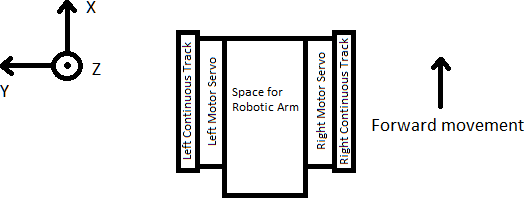
\includegraphics[width=\linewidth]{sections/assets/Mobile_platform_paint_text3_horiz.PNG}
    \caption{The Mobile Platform seen from above.}
    \label{Mobile_platform_paint}
\end{figure}


\begin{figure}[h]
    \centering
    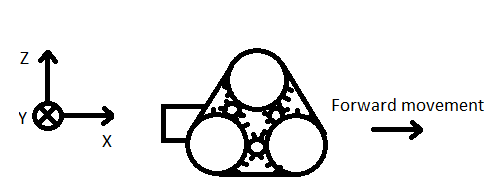
\includegraphics[width =\linewidth]{sections/assets/Band_platform_coordinates.PNG}
    \caption{The Mobile Platform seen from the side of one track.}
    \label{Band_platform_coordinates}
\end{figure}

\subsubsection{Trailer}
In order to get power to each motor servo and the Raspberry Pi, two battery packs with 8 batteries in each were used. Since these battery packs together with the Raspberry Pi and the two BrickPi motorshields were to large to place on the mobile platform, a trailer was built and mounted behind the platform with the devices stacked on it. The trailer can be seen attached to the mobile platform in Fig.~\ref{Trailer}.

\begin{figure}[h]
    \centering
    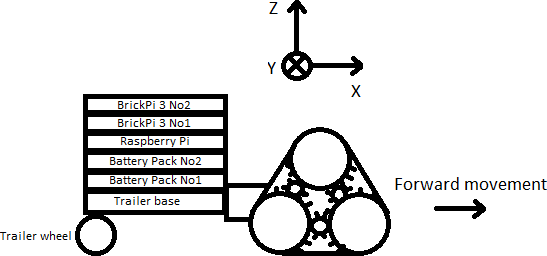
\includegraphics[width =\linewidth]{sections/assets/Trailer.PNG}
    \caption{The Mobile Platform seen from the side of one track.}
    \label{Trailer}
\end{figure}

\subsection{Line follower}

The docking sequence of the robots movement was implemented using a line follower. A QTRX reflectance sensor from Pololu was used together with a black line to guide the robot close to the factory and to stop it with a perpendicular angle to the factory. During the project, there occurred a connection issue between the Raspberry Pi and the sensor array due to the fact that  NixOS could not handle the incoming data. This issue was resolved by buying an additional breakout board which, in turn, had its own GPIO pins and at the same time could be connected with the Raspberry Pi 3 through another medium, in this case via a usb-cable. The breakout board used in this project was the Adafruit FT232H Breakout.

\subsubsection{Adafruit FT232H breakout}
Adafruit FT232H Breakout is a breakout board from Adafruit which contains the F232H chip from FTDI and has has one port each for a usb c and stemma qt male connectors. The board is also equipped with 16 GPIO pins and also has the ability to speak with many protocols including SPI, ITC, serial UART, JTAG and others. In the project, this board was used to transfer GPIO singals from individual sensor on a sensor array to the Raspberry Pi computer.
\begin{figure}[h]
    \centering
    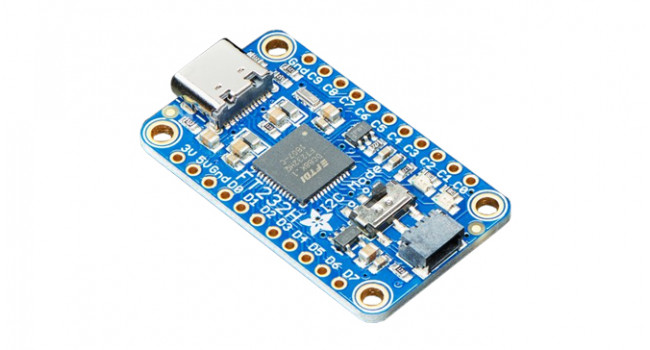
\includegraphics[width =\linewidth]{sections/assets/FT232H.jpg}
    \caption{FT232H Breakout.}
    \label{FT232H}
\end{figure}

\subsubsection{Sensor Array}
The Sensor array used in this project was a QTRX-MD-16A Reflectance array from Pololu. Each sensor on the sensor array is made from a photo transistor and paired with an IR-led which powers on and keeps emitting light while the sensor array module is powered on. The signal from the photo transistor is transmitted as an analog voltage from the sensor array.
\begin{figure}[h]
    \centering
    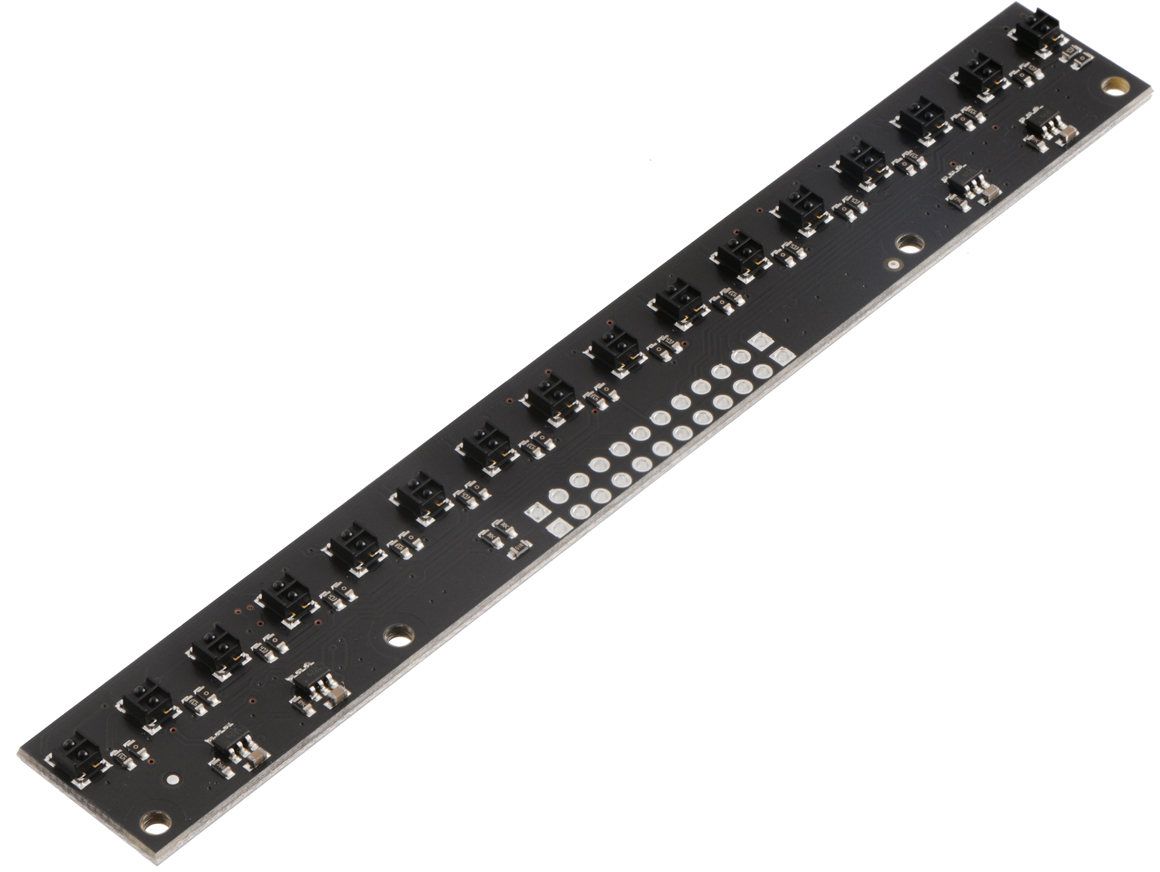
\includegraphics[width =\linewidth]{sections/assets/Sensor_array.jpg}
    \caption{QTRX-MD-16A.}
    \label{Sensor_array}
\end{figure}
\subsubsection{Implementation of routine}
As mentioned earlier, the signal from the sensor array was transmitted through the breakout board to the Rapberry Pi, this signal included the state of each photo transistor. The state of each transistor is being displayed as TRUE if the black line is underneath it and FALSE if the transistor only detects a white surface underneath. Since a pre-owned sensor array was used, only 4 functioning photo transistor/LED pairs that were close to each other were available, limiting the line following procedure to 4 reference points. More reference points may have proven to be more optimal in the case whit sharp angles and faster speeds. However the fact that the line only triggers 2 or less reference points at each time, made us determine that the sensor array was good enough for the given task.

The position of the line underneath the sensor array was determined by setting a weight on each photo transistor. The weights of each sensor corresponded to its position from the leftmost position in the robot's forward direction to the rightmost position, giving the weight of the first sensor the value of 1 and the weight of the fourth sensor the value of 4. By summing all weights from the transistors that detected the line and dividing this value with the number of transistors that detected the line, a mean value of the active weights can be derived, see Fig.~\ref{Line_Position}. M is the mean value of the weights of transistors that detected the line. The value of each Sn is 1 if the transistor detecteda line underneath it or 0 if a white surface was detected.
\begin{equation}
    M=\frac{1*S1+2*S2+3*S3+4*S4}{S1+S2+S3+S4}
    \label{Line_Position}
\end{equation}

When the line is perpendicular to the mobile platform and underneath the two middle photo transistors, the mean value will be 2.5. This value is determined as the reference value of the sensor array, we denote it by R, whenever the mean value from the sensor array will be different from it, power will be added to one motor servo in the mobile platform and reduced from the other motor servo in the platform. The difference between the reference and the mean value of the sensor array will be called the error, see eq.
\begin{equation}
    E=R-M
    \label{Error_Position}
\end{equation}

An example of the how the error is calculated using Eq.~\eqref{Line_Position} and \eqref{Error_Position} together with data from the diodes can be seen in Fig.~\ref{Line_Error_ex}

\begin{figure}[h]
    \centering
    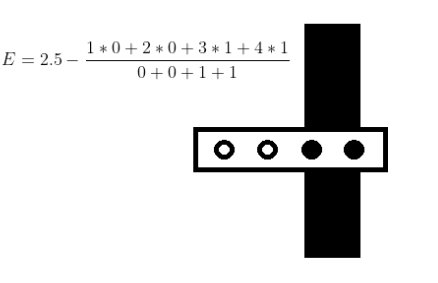
\includegraphics[width =\linewidth]{sections/assets/Line_Error_ex.PNG}
    \caption{Calculation of the error in the case where the two phototransistors on the right are detecting the line}
    \label{Line_Error_ex}
\end{figure}


By creating a controller with the purpose of minimizing the error, the robot will be controlled to follow the line.

\subsection{Robot arm}
A simplified model of the robot arm can be seen in Fig.~\ref{Arm_model} where the measured distances from \(d_1\) to \(d_7\) and the vertical angle Theta can be seen. in Fig.~\ref{arm_overview} an overview of the robot model can be seen showing how the angle beta was specified.
\begin{figure*}[h]
    \centering
    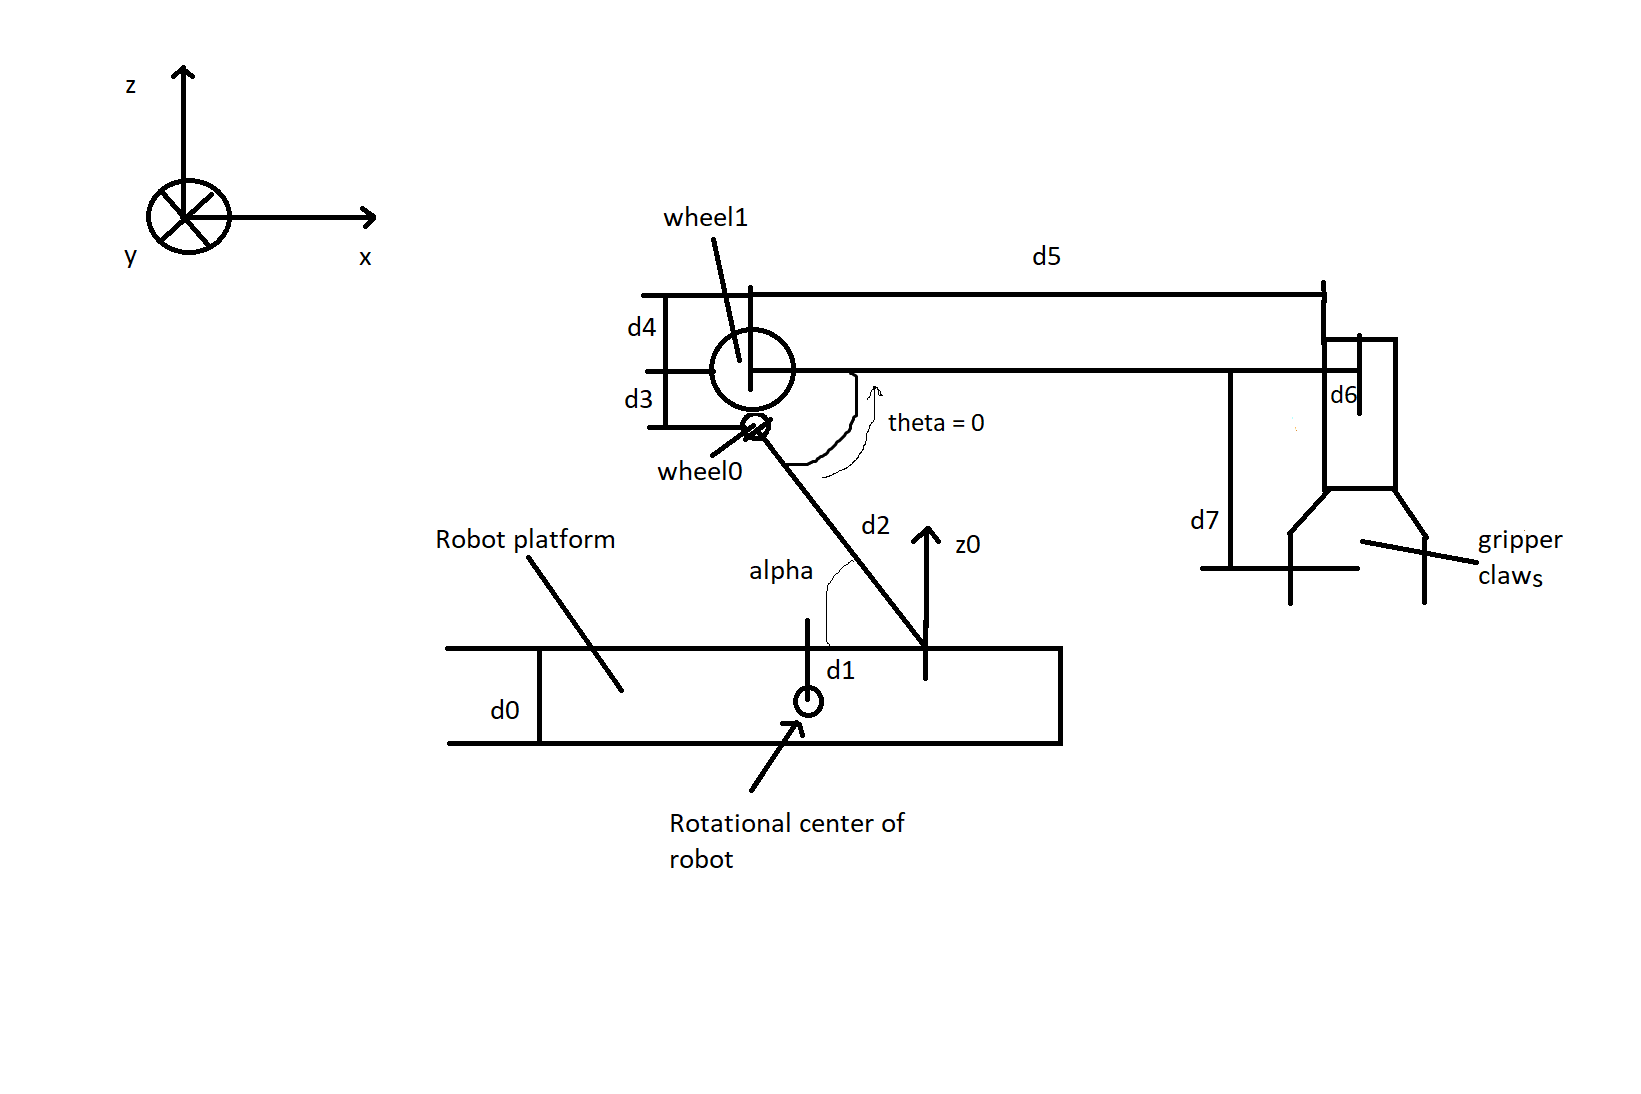
\includegraphics[width=\linewidth]{sections/assets/Arm_model.png}
    \caption{Arm model side view.}
    \label{Arm_model}
\end{figure*}
\begin{figure}[h]
    \centering
    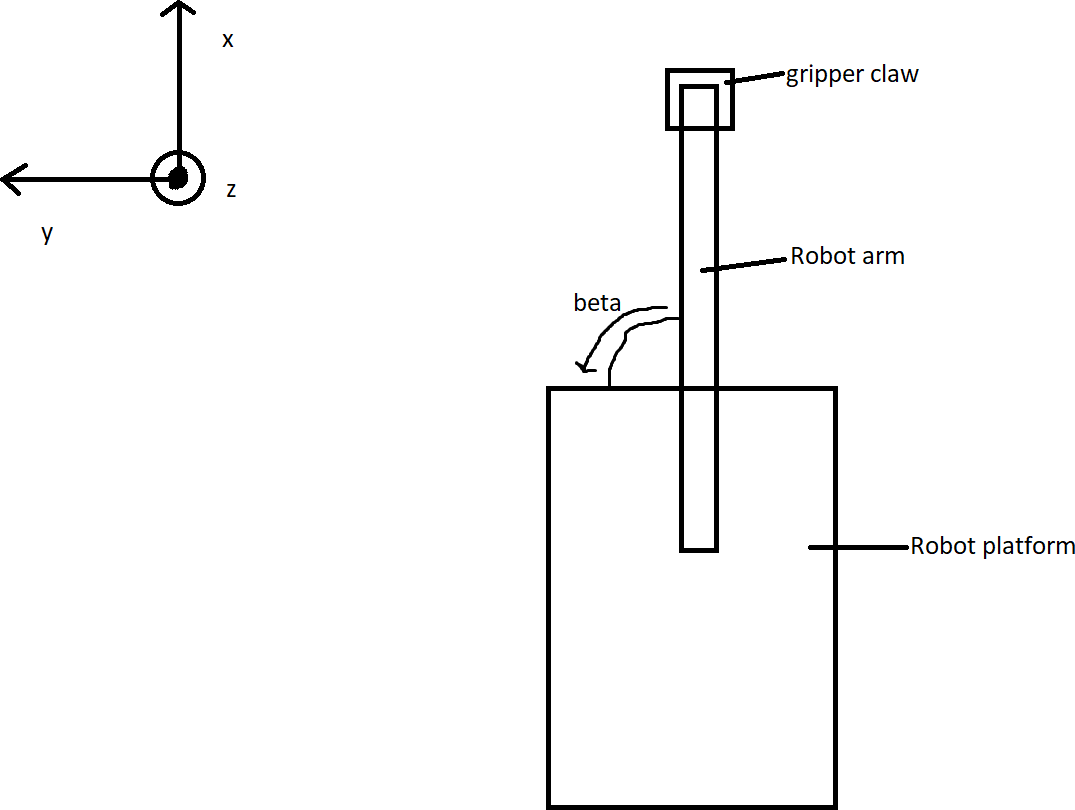
\includegraphics[width=\linewidth]{sections/assets/Arm_overview.png}
    \caption{Arm model overview.}
    \label{arm_overview}
\end{figure}
The robot arm can rotate in the xy-plane around the \(z_0\) axis which can be seen in Fig.~\ref{Arm_model} with a angle Beta using a EV3 large servomotor mounted inside the base of the robot. The upper part of the robot, from wheel1 to the gripper claw can also rotate vertically in the xz-plane using another EV3 large servomotor mounted between wheel0 and the point on the base from where the axis \(z_0\) is originating. The gripper claws  driven with a EV3 servo motor medium since it weighs less. The distances \(d_0\) to \(d_7\) was measured with a ruler and can be seen in table \ref{Tab:distance_table}
\begin{table}[h]
\begin{center}
\begin{tabular}{ |c|c| }
 \hline
 \(d_0\) & 8 cm  \\
 \(d_1\) & 1.5 cm  \\
 \(d_2\) & 11.7 cm  \\
 \(d_3\) & 2.2 cm\\
 \(d_4\) & 2.2 cm\\
 \(d_5\) & 23.5 cm\\
 \(d_6\) & 1.5 cm\\
 \(d_7\) & 11 cm \\
 \hline
\end{tabular}
\end{center}
\caption{Table of measured distances \(d_1\) to \(d_7\).}
\label{Tab:distance_table}
\end{table}
\subsubsection{Forward kinematics}
To be able to describe where in the world the gripper claw is, a problem often refereed to as the forward kinematics problem \parencite{Spong2004} had to be solved. This was used with a series of homogeneous transformations each representing a change in position and/or orientation relative to what is usually referred to as a frame. The first homogeneous transformation was from the level of the floor to the top of the robot platform, with a distance \(d_0\) which can be seen as a pure translation in the z-direction and can be described as Eq.~\eqref{T01} as according to \parencite{Spong2004}.
\begin{equation}
    T_{01} =
    \begin{bmatrix}
    1&0&0&0\\
    0&1&0&0\\
    0&0&1&d_0\\
    0&0&0&1\\
    \end{bmatrix}
    \label{T01}
\end{equation}
then a transformation between the rotational center of the robot to where link \(d_2\) is connected to the base of the robot, which can be expressed as a pure translation in the x-direction. This can be seen in Eq.~\eqref{T12}
\begin{equation}
    T_{12} =
    \begin{bmatrix}
    1&0&0&d_1\\
    0&1&0&0\\
    0&0&1&0\\
    0&0&0&1\\
    \end{bmatrix}
    \label{T12}
\end{equation}
followed by a transformation from the beginning of link \(d_2\) to the center of wheel0. This was done by first making a pure rotation around the z-axis with a angle beta, after which a pure translation in the z-direction with a distance \(d_2\cdot sin(\pi-alpha)\) was made, followed by a translation in the x-direction with a distance \(d_2\cdot cos(\pi - alpha)\) as can be seen in Eq.~\eqref{T23}
\begin{equation}
    T_{23} =
    \begin{bmatrix}
    cos(beta)&-sin(beta)&0&0\\
    sin(beta)&cos(beta)&0&0\\
    0&0&1&0\\
    0&0&0&1\\
    \end{bmatrix}
    \cdot
    \begin{bmatrix}
    1&0&0&0\\
    0&1&0&0\\
    0&0&1&d_2\cdot sin(\pi-alpha)\\
    0&0&0&1\\
    \end{bmatrix}
    \cdot
    \begin{bmatrix}
    1&0&0&d_2\cdot cos(\pi-alpha)\\
    0&1&0&0\\
    0&0&1&0\\
    0&0&0&1\\
    \end{bmatrix}
    \label{T23}
\end{equation}
this was followed by a translation in the z-direction of the distance \(d_3\) between the center of wheel0 to the center of wheel1, see Eq.~\eqref{T34}
\begin{equation}
    T_{34} =
    \begin{bmatrix}
    1&0&0&0\\
    0&1&0&0\\
    0&0&1&d_3\\
    0&0&0&1\\
    \end{bmatrix}
    \label{T34}
\end{equation}
after which a rotation of the coordinate frame in the center of wheel1 was made by an angle -theta around the y-axis and then a translation in the x-direction of the frame in wheel1 by a distance \(d_5 + d6\), see Eq.~\eqref{T46}
\begin{equation}
    T_{46} =
    \begin{bmatrix}
    cos(-theta)&0&sin(-theta)&0\\
    0&1&0&0\\
    -sin(-theta)&0&cos(-theta)&0\\
    0&0&0&1\\
    \end{bmatrix}
    \cdot
     \begin{bmatrix}
    1&0&0&d_5 + d_6\\
    0&1&0&0\\
    0&0&1&0\\
    0&0&0&1\\
    \end{bmatrix}
    \label{T46}
\end{equation}
due to the mechanics of the robot model the gripper claw is always pointing straight downwards independent of the angle theta, therefore the coordinate system in the middle if the medium motor connected to link \(d_5\) was rotated back with a positive angle theta before it was translated a distance \(-d_7\) in the z-direction as can be seen in Eq.~\eqref{T67}
\begin{equation}
    T_{67} =
    \begin{bmatrix}
    cos(theta)&0&sin(theta)&0\\
    0&1&0&0\\
    -sin(theta)&0&cos(theta)&0\\
    0&0&0&1\\
    \end{bmatrix}
    \cdot
     \begin{bmatrix}
    1&0&0&0\\
    0&1&0&0\\
    0&0&1&-d7\\
    0&0&0&1\\
    \end{bmatrix}
    \label{T67}
\end{equation}
the expression of where the gripper claw can be then expressed as in Eq.~\eqref{T_tot} where both it's position and orientation relative to the robot platform is described.
\begin{equation}
    T = T01\cdot T12\cdot T23 \cdot T34 \cdot T46 \cdot T67
    \label{T_tot}
\end{equation}
\subsubsection{Inverse kinematics}
After being able to describe the position and orientation of the gripper it was necessary to have a way of calculating the desired angles theta and beta of the arm to get the gripper claw to a desired position. This problem is often referred to as the inverse kinematics problem. For this robot the angle theta was directly determined by the height of the desired gripper claw position which was calculated according to Eq.~\eqref{inv_theta_calc_1} to \ref{inv_theta_calc_5} and the distances \(h_1\) to \(h_3\) can be seen in Fig.~\ref{inv_theta_img}
\begin{figure}[h]
    \centering
    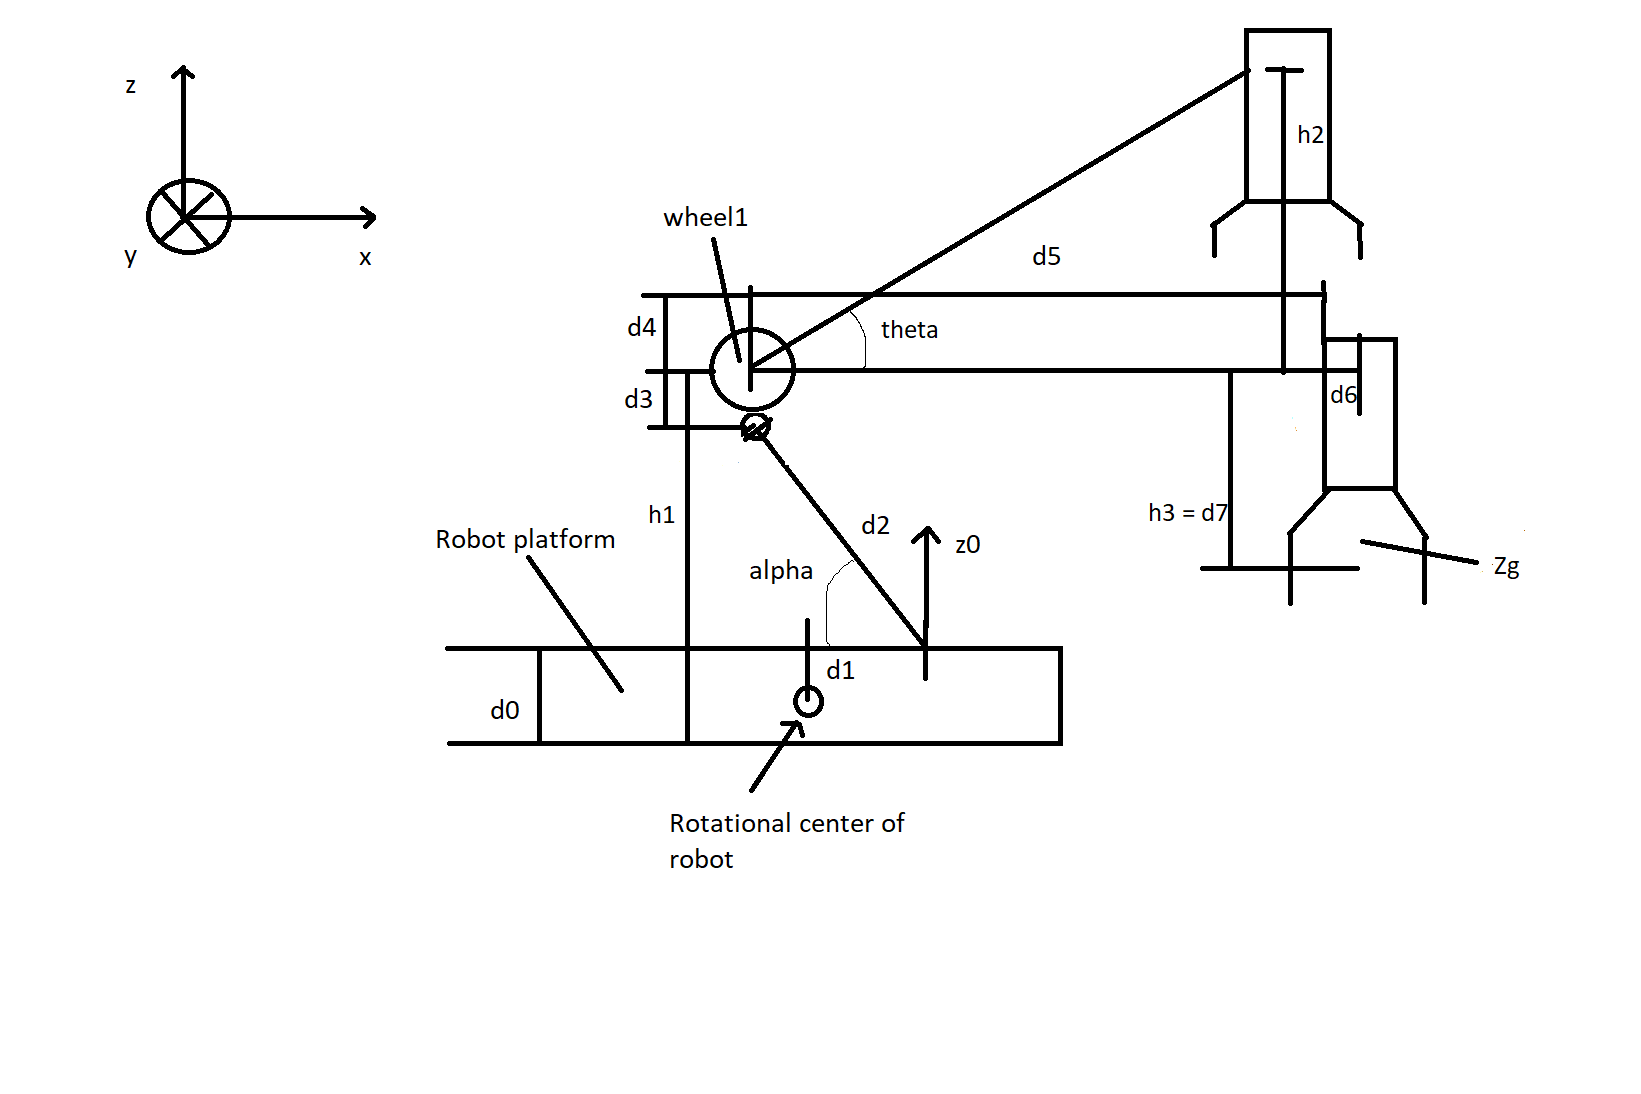
\includegraphics[width=\linewidth]{sections/assets/Arm_model_inv_theta.png}
    \caption{distances \(h_1\) to \(h_3\) on arm model.}
    \label{inv_theta_img}
\end{figure}
\begin{equation}
    Z_g = h_1+h_2 - h_3
    \label{inv_theta_calc_1}
\end{equation}
and from Fig.~\ref{inv_theta_img} it can be seen that
\begin{equation}
    h_1 = d_2 \cdot sin(alpha)
    \label{inv_theta_calc_2}
\end{equation}
\begin{equation}
    h_2 = (d_5 + d_6) \cdot sin(theta)
    \label{inv_theta_calc_3}
\end{equation}
\begin{equation}
    h_3 = d_7
    \label{inv_theta_calc_4}
\end{equation}
substituting \(h_1\) to \(h_3\) with expressions from Eq.~\eqref{inv_theta_calc_2} to \eqref{inv_theta_calc_4} the final expression for the angle theta can be solved for in the way that can be seen in Eq.~\eqref{inv_theta_calc_5}
\begin{equation}
    theta = sin^{-1}(\frac{Z_g - d_2 \cdot sin(alpha) + d7}{(d_5 + d_6)})
    \label{inv_theta_calc_5}
\end{equation}
Since the arm could rotate horizontally it could reach points on a circle, see Fig.~\ref{inv_beta_radius_img}, around itself where the radius of that circle, with the rotational center of the robot being the center of the circle, depended on the angle theta in a way that is described in Eq.~\eqref{beta_radius_eq}.
\begin{figure}[h]
    \centering
    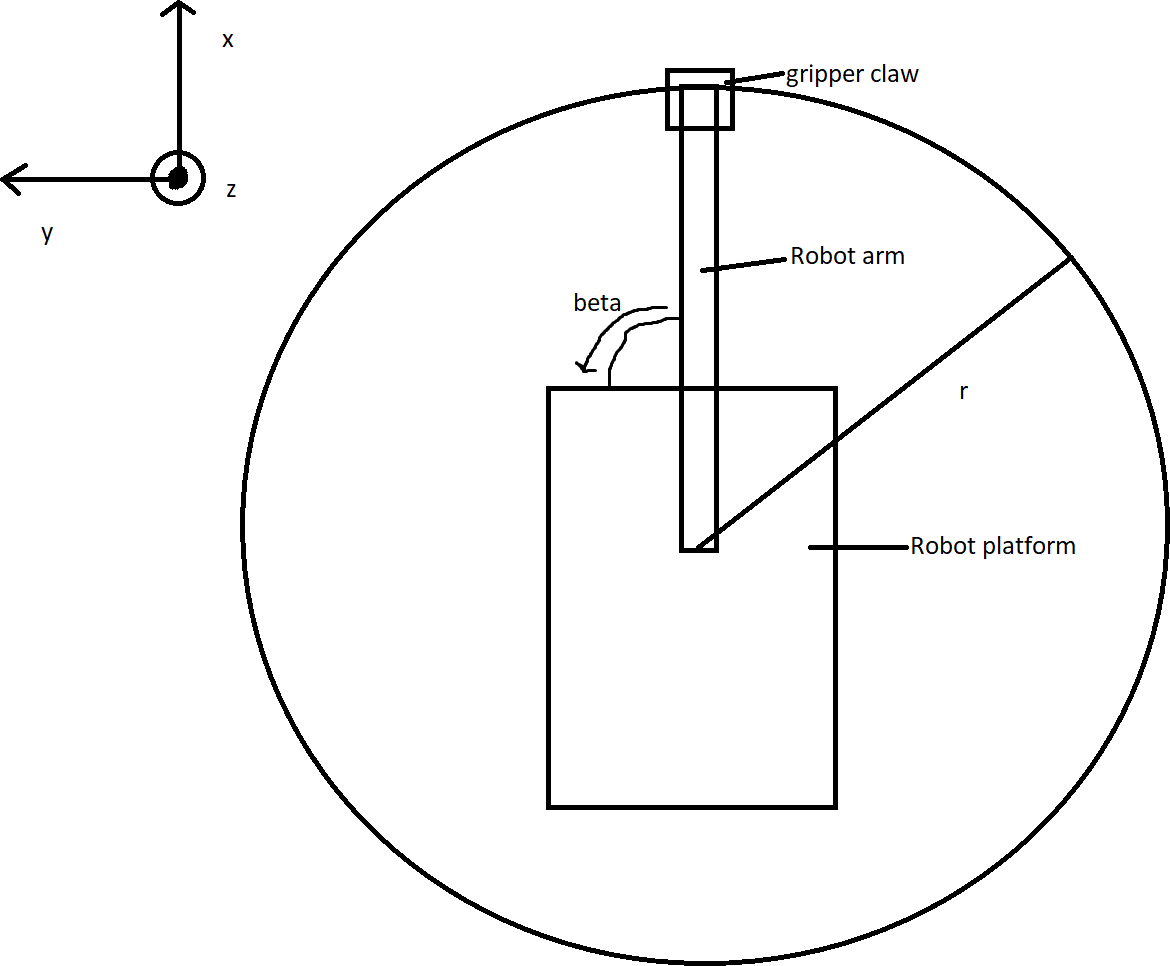
\includegraphics[width=\linewidth]{sections/assets/inv_beta_radius.png}
    \caption{distances \(h_1\) to \(h_3\) on arm model.}
    \label{inv_beta_radius_img}
\end{figure}
\begin{equation}
    r = (d_5 + d_6)\cdot cos(theta) - d_2\cdot cos(alpha) + d_1
    \label{beta_radius_eq}
\end{equation}
calculations of x and y positions on a circle can be seen in Eq.~\eqref{circle_x} and \eqref{circle_y}
\begin{equation}
    x = r\cdot cos(beta)
    \label{circle_x}
\end{equation}
\begin{equation}
    y = r\cdot sin(beta)
    \label{circle_y}
\end{equation}
substituting r to the expression from Eq.~\eqref{beta_radius_eq} the calculations of the x and y positions on the circle around the robot can be seen in Eq.~\eqref{circle_x_robot} and \ref{circle_y_robot}
\begin{equation}
    x = ((d_5 + d_6)\cdot cos(theta) - d_2\cdot cos(alpha) + d_1)\cdot cos(beta)
    \label{circle_x_robot}
\end{equation}
\begin{equation}
    y = ((d_5 + d_6)\cdot cos(theta) - d_2\cdot cos(alpha) + d_1)\cdot sin(beta)
    \label{circle_y_robot}
\end{equation}
solving for beta Eq.~\eqref{circle_x_robot} and Eq.~\eqref{circle_y_robot} the following expressions was achieved
\begin{equation}
    beta = cos^{-1}(\frac{x}{(d_5 + d_6)\cdot cos(theta) - d_2\cdot cos(alpha) + d_1})
    \label{Beta_x_robot}
\end{equation}
\begin{equation}
    beta = sin^{-1}(\frac{y}{(d_5 + d_6)\cdot cos(theta) - d_2\cdot cos(alpha) + d_1})
    \label{Beta_y_robot}
\end{equation}
these two expressions both have a denominator which is equal to zero for an angle \(theta = \pm \frac{\pi}{2}\), two angles that the robot can never reach due to the way the Lego hardware is put together.
From Eq.~\eqref{Beta_x_robot} and Eq.~\eqref{Beta_y_robot} it is clear that only the desired x or the y position was needed to calculate beta, in this project the x positions were used.
\subsubsection{Resolution}
As mentioned before the motors used in the robot arm was two Lego EV3 servo motor large for making the arm move vertically and horizontally and one Lego EV3 servo motor medium inside the gripper to pick up boxes on the miniature industry platform. Both the Large and the medium motors had a resolution of 1 degree, meaning the motors gives 360 readings on one revolution. Also on the robot the cogwheel attached to the motor controlling vertical movement on the arm, see wheel0 in Fig.~\ref{Arm_model}, was connected to another cogwheel, see wheel1 in Fig.
~\ref{Arm_model}, which had 5 times as many teeth giving 5 times higher resolution for the arm itself than the motor in vertical movement. In the same way the cogwheel attached to the motor controlling horizontal movement of the arm was connected to another cogwheel with 3 times as many teeth giving 3 times higher resolution for the arm relative to the motor in horizontal movement.
\subsubsection{Initialization}
There is no memory in the motors which makes the robot unaware of the original orientation of the arm on boot. Therefore an initialization process was made for the robot using two Lego EV3 touch sensors. On boot the robot moved the arm with constant angular speed, in the beta direction, until a lego piece, moving with the arm, pressed one of the touch sensors at \(beta = -90^{\circ}\) then it stopped moving in that direction. In the same way the robot moved the arm in the positive theta direction until another lego piece getting closer to the other touch sensor with an increasing beta angle, pressed the second touch sensor at \(theta = 36^{\circ}\). then it stopped in that direction. At the point when both touch sensors was pressed and the arm had stopped moving in both directions the position of the arm was known.
\subsection{Robot software}
Two BrickPi3 motor shields were used to drive the motors and sensors on the robot. A complete library for controlling lego motors and sensors connected to the motor shields were developed by the manufacturers of the BrickPi3 together with the shields and was used to control the motors. Additionally P, PI and PID controllers was developed in this project to compare functions in the BrickPi3 library for controlling the motors and the movement on the arm.
\subsubsection{P controller}
A P controller, or proportional controller, is a feedback control structure where the output error is fed back to the motors to make them act proportional to the error. In the P controller made for controlling the movement on the robot arm an angular error was expressed, see Eq.~\eqref{ang_err}
\begin{equation}
    e_{\theta} = \theta_{desired} - \theta
    \label{ang_err}
\end{equation}
where \(\theta\) is the current angular position of the arm and \(\theta_{desired}\) is the goal angle. The angular error was then fed back to the motors to make them act on it is a way that can be seen in Eq.~\eqref{P_control}
\begin{equation}
    P = K_p\cdot e_{\theta}
    \label{P_control}
\end{equation}
where P is motor speed, proportional to the angular error and \(K_p\) is a proportional gain which determines how aggressive the controller should be.

\subsubsection{PI controller}
A PI controller or proportional integral controller is a proportional controller to which a term which integrates the error over time is added. The integration was done in a discrete fashion where, in every loop of the robot arm code running, the new calculated error was added to a integral error term, see Eq.~\eqref{integral_term}
\begin{equation}
    e_{integral} = e_{integral} + e_{\theta}
    \label{integral_term}
\end{equation}
where \(e_{integral}\) is the discrete approximation of the integrated error, \(e_{\theta}\) is the same as in Eq.~\eqref{ang_err}. This error was adding up over time and the feedback to the motors can be seen in Eq.~\eqref{PI_control}
\begin{equation}
    P = K_p\cdot e_{\theta} + K_i\cdot T_s\cdot e_{integral}
    \label{PI_control}
\end{equation}
where P is the motor speed, \(T_s\) is the sampling period of the code to make the integral term normalized in a sense, and \(K_i\) is the integral gain which determines how much the motors should act on the integral error.

\subsubsection{PID controller}
A PID or proportional integral derivative controller is a control structure where both a proportional, integral, and a derivative term is added. The differentiation was also done in a discrete fashion and was approximated as in Eq.~\eqref{derivative_term}
\begin{equation}
    e_{diff} = e_{old} - e_{\theta}
    \label{derivative_term}
\end{equation}
where \(e_{diff}\) is the discrete approximation of the differentiated error, \(e_{old}\) is the old error from the previous loop of the code and \(e_{\theta}\) is the same as in Eq.~\eqref{ang_err}. The feedback to the motors was done according to Eq.~\eqref{PID_control}
\begin{equation}
    P = K_p\cdot e_{\theta} + K_i\cdot e_{integral} + K_p\cdot e_{diff}
    \label{PID_control}
\end{equation}
\subsubsection{Tuning of the controllers}
The tuning of the controllers was made with a Ziegler Nichols approach \parencite{FeedbackControl}, since a development of a dynamic model of the arm was not completed. The Ziegler Nichols tuning method required two measured parameters to be found. First the Oscillation gain which is the gain of a proportional controller \(K_p\) for which the output of the system acting on a step response is undamped oscillations. This was found by making the robot arm act on a step response several times while changing the value of the proportional gain \(K_p\). The second measured parameter is the oscillation time \(T_{osc}\), e.g the time it takes for the system to make one undamped oscillation period. This was found by looking at a plotted graph of the undamped oscillations and counting the measured values in one period. The calculations of the oscillation time could then be done as shown in Eq.~\eqref{osc_time}
\begin{equation}
    T_{osc} = n\cdot T_s
    \label{osc_time}
\end{equation}
where \(T_{osc}\) is the oscillation time, n is the number of measured values in one undamped oscillation period from the output of the step response and \(T_s\) is the sampling period of the robot.

\subsubsection{Controller for line following}
The same operating speed was chosen for both the right and left track of the mobile platform, the speed of each track would not change from the operating speed as long as Error calculated in Eq.~\eqref{Error_Position} would remain zero. If the position of the line underneath the sensor array changed, the error would grow and the speed of both tracks would change. An architecture for the controller which minimizes the error could be observed in fig.

\begin{figure}[h]
    \centering
    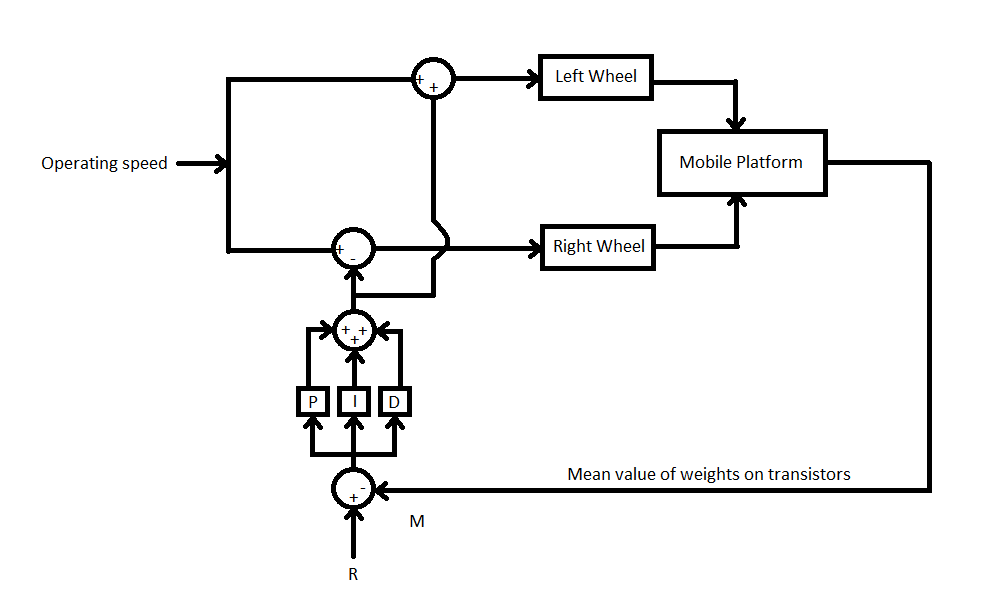
\includegraphics[width=\linewidth]{sections/assets/Control_system1.PNG}
    \caption{Block diagram of the PID controller constructed for the line following procedure}
    \label{Control_system1}
\end{figure}

\subsection{Software nodes}
\label{sec:nodes}
% What is a software node?
The usage of LCM allows us to define ``software nodes'' which were briefly explained in section~\ref{sec:ROS}.
A software node is a small stand-alone executable program, written in any language that usually has a single purpose in the system the project implements.
For example, one node in the system reads data from the DWM;
another approximates its position using a Kalman filter;
another actuates the motors to pick up the object the system aims to displace; etc.
If a node depends on data from another node,
it is packaged in a message of a certain type and published on a channel.
The depending node then subscribes to this channel,
receives a message whenever one is published on that channel,
and processes it.

% How do the structure of nodes help?
This structure have allowed us to write a set of smaller programs which are usually easier to implement and debug across multiple project members,
instead of maintaining a monolithic program that does everything, which are usually harder to both implement and debug,
especially when multiple project members need to contribute.


% Here we'll summarize each node
Each node in the project follow the naming scheme of \texttt{lcm-<type>-<desc>.<ext>} where
\begin{description}
\item[\texttt{<type>}] denotes the type of three possible alternatives:
  \texttt{source}, which denotes that the node only provides messages to the system;
  \texttt{sink}, only receives messages from the system; and
  \texttt{int} (for `intermediate'), both receives and generates messages.
\item[\texttt{<desc>}] is a list of words interspaced by a \texttt{-} that provide a short description of the node's purpose.
\item[\texttt{<ext>}] is the source file extension. It describes how the node should be built before it can be executed.
  For example, if the extension is \texttt{c} then the node was written and C and needs to be compiled and linked with a C compiler before the resulting binary can be executed.
  If the extension instead is \texttt{py} then the node was written in Python, and nothing must be done before the script can be executed,
  except for satisfying the script's dependencies.
\end{description}

The source files for all nodes can be found in \texttt{src/}.

Fig.~\ref{fig:node-schema} contains a visualization of all system nodes and with which other nodes they talk to.
Communication occurs over a common LCM channel name where only one message type is expected on each channel.
The massage type can be derived from the channel name, and vice versa.
This was done for sake of simplicity.

\begin{figure}[h]
  \centering
  \begin{tikzpicture}[
    node distance = 2cm,
    auto,
    ]
    % input nodes
    \node[block] (arrowhead) {Arrowhead};
    \node[block, left of=arrowhead] (enc) {motor \\ encoders};
    \node[block, left of=enc] (dwm) {DWM};
    \node[block, right of=arrowhead] (line-follower) {line \\ follower};

    % intermediate nodes
    \node[block, yshift=-6cm] at ($(enc)!0.5!(arrowhead)$) (master) {master};
    \node[block, yshift=-2cm] at ($(dwm)!0.5!(enc)$) (kalman) {Kalman \\ filter};
    \node[block, below of=kalman] (state) {system \\ state};

    % % robot modes
    \node[block, below of=master] (object-mode) {Object \\ mode};
    \node[block, left of=object-mode, xshift=-2em] (dwm-mode) {DWM \\ mode};
    \node[block, right of=object-mode, xshift=2em] (line-mode) {Line-follow \\ mode};

    \path[<->] (kalman) edge (state)
    (master) edge (object-mode);
    \path[->] (dwm) edge (kalman)
    (enc) edge (state)
    (state) edge (dwm-mode)
    (state) edge (master)
    (master) edge (dwm-mode)
    (master) edge (line-mode)
    (line-follower) edge (master)
    (line-follower) edge (line-mode)
    (enc) edge (object-mode)
    (arrowhead) edge (master);
  \end{tikzpicture}
  \caption{Relation chart over the system's nodes.}
  \label{fig:node-schema}
\end{figure}

All system nodes (and the source files under \texttt{src} which define them) are described below.
\begin{description}
\item[DWM node (\texttt{lcm-source-dwm.c})]
This node is responsible for extracting the position and acceleration data from the DWM.
Upon execution it opens opens a serial communication to the DWM, enters the shell mode and allocates a buffer into which received data is read into.
Afterwards it enters a loop within which the shell command \texttt{av} is continuously called.
While spinning in this loop, the node keeps the time and ensures that the command \texttt{apg} is called with a frequency of $10$~Hz.
After the execution of each command:
\begin{enumerate}
  \item the response is read into the buffer;
  \item the buffer is parsed for data of interest;
  \item data is converted to SI units --- m for position coordinates, $\text{ms}^{\text{-2}}$ for acceleration; and
  \item an appropriate message type is constructed and published unto either the \texttt{IO\_POSITION} or \texttt{IO\_ACCELERATION} channel.
\end{enumerate}

\item[Motor encoders node]

\item[Arrowhead node (\texttt{lcm-source-arrowhead.py})]
  This node is responsible for listening on requests from the service provider and publish the message in LCM.
  The node is running a flask application which is listening on the service provider.
  To trigger the functions in the flask application a specific URL is required.
  The functions is then forwarding the messages to other nodes through LCM.
  It publish a message action; ``pick up'' or ``place'', and position; ``right'' or ``left''.

  The flask runs in http which is insecure.
  The secure mode (https) is not needed because the call for the URL is happening in the same device as the arrowhead node is running on.

\item[Line follower node]

\item[Kalman filter node (\texttt{lcm-int-dwm-filter.py})]

\item[System state node (\texttt{lcm-int-system-state.py})]
This node takes the filtered DMW data and the the motor encoders data and estimate the new position, as described in \eqref{eq:Disc_EOM}.
By knowing the old positions, the new positions and the elapsed time (sampling time) it is also possible to estimate the velocities.
The $x$ and $y$ velocities are required for Kalman filter to be able to make better estimations for the spacial position.
This node also estimate the angle of attack and its derivative, i.e. the angular velocity.


\item[Master node (\texttt{lcm-int-master.py})]
  As seen in Fig.~\ref{fig:state_machine}, the system's behavior can be described as a finite state machine.
  The master node is responsible for ensuring that the correct mode node (DWM, object or line-follow) is running at the right time,
  and thus implements the referenced state machine description.
  For example, before switching to line-follow mode, the system current state is compared to a set of points where the robot would be close enough to a station to find a line.
  If it is found that the system is too far away, the line-found event is ignored and logged to \texttt{stderr} for debugging purposes.

\item[DWM mode node (\texttt{lcm-DWM-drive.py})]
This is the node where the current position $(x, y, \theta)$ and the desired position are the inputs.
By having this inputs it is possible to calculate the angular and spacial errors for the movement, as described in \eqref{eq:cart2polar}
Two simple PID controllers are designed to make sure this errors go to zero, as shown in fig\ref{fig:PID1} and fig\ref{fig:V_PID}.
The robot has arrived to the desired position when the errors are zeros.

\item[Object mode node]

\item[Line-follow mode node]

\end{description}

Some debugging nodes are also defined, but are external from the system-internal relations displayed in Fig.~\ref{fig:node-schema}:
\begin{description}
\item[Message spoofer (\texttt{lcm-debug-spoof-message.py})]
  While developing nodes it is useful to ensure that it responds to LCM messages in the expected manner.
  Instead of writing an ad-hoc node that sends whatever messages that need to be tested,
  this node allows the developer send a message of any type by just specifying the correct parameters.

  % Describe how the node works? Inspects the LCM-generated Python module.

  For example, to send a message indicating that the Kalman-filtered position of the system is at the coordinates $(4.23, 5.12)$,
  execute \texttt{lcm-debug-spoof-message.py KALMAN\_POSITION 4.23 5.12}.

\item[Message sink (\texttt{lcm-debug-print-all.py})]
  An inverse of the above debug node: instead of sending a message of any type,
  this node prints a message of any type.
  Useful for inspecting the system as any and all LCM messages will be printed by first subscribing to all channels.
\end{description}

\subsection{Arrowhead clients}

\begin{figure*}[h]
	\centering
	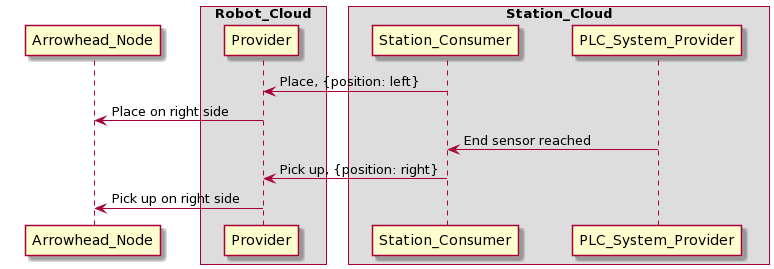
\includegraphics[width=\linewidth]{sections/assets/arrowhead_sequence_diagram.png}
	\caption{The communication between clouds and the arrowhead node.}
	\label{fig:arrowhead_intercloud}
\end{figure*}

Fig.~\ref{fig:arrowhead_intercloud} shows the inter-cloud communcation and communication to the Arrowhead node.
The Station Consumer sends a POST request for the ``place'' service and also sends a json with the position.
The provider is then sending a GET request depending on the service and the position to the arrowhead node.
When Arrowhead node receives the request, it will publish a message which other nodes are getting if they are subscribed to that channel.

When the robot have executed the service, the conveyor belt sensor detects a piece on the conveyor belt and starts running.
When it reaches the end sensor, the conveyor belt will stop and will notify the Station Consumer which will then send a request for the ``pick up'' services with a position.
The request will then reach the robot and it will execute the service.

\subsubsection{Provider}
The purpose of the provider is to provide services which a consumer in the same arrowhead cloud or in another arrowhead cloud can consume. The provider is offering two services; ``pick up'' and ``place''.
When running the provider it registers the system and its services to the Service Registry.

The provider is using a secure https connection with self signed client certificate.
The security of Arrowhead Framework is relying on SSL Certificate Trust Chains.
The chain consist of three layers; Master certificate, Cloud certificates and Client certificates.
The cloud certificate is created and signed from a master certificate's private key.
The client certificates are created and signed from a cloud certificate' private key.
In that way the whole chain is trustworthy. (\url{https://github.com/eclipse-arrowhead/core-java-spring})

The service functions in the provider is using POST http-method.
When sending a request for a service, a json with the position where it should pick up is required.
When the provider recieves a post request with a position, the provider is then sending a request to the lcm-source-arrowhead.py so called arrowhead node.
The arrowhead node is then publishing a message to other nodes with a timestamp, ``pick up'' or ``place'' and position.

The provider can either be running on the raspberry pi where the nodes are running or on another machine.
If running on another machine a ssh connection is needed to communicate with the rasberry pi.
The purpose of a ssh connection is to communicate with the arrowhead node in a secure way.
SSH is a secure network protocol which encrypts messages that are going through the SSH connection.

To allow other consumers to ask for services the provider is offering, intra- or inter-cloud is needed.
Intra-cloud rules is needed if consumer is in the same cloud.
If the consumer is in another cloud, inter-cloud rules need to be added.
The intra and inter-cloud rules can be added in the Authorization system.

The provider are using the client-library-python and is written in Python.

\subsubsection{Consumer}
The purpose of the consumer is to consume services which are offered by a provider in Arrowhead Service Registry.
The consumer needs to manually be added as a system to the Service Registry and have intra- or inter-cloud rules for the services it want to consume.

The consumer in the project were used for debuging and testing the provider. The sequence diagram in Fig.~\ref{fig:arrowhead_intercloud} shows the real system and the communication between. The Station Consumer is instead communicate with the provider.
The consumer is using self signed certificates in the https connection which is the same as the provider.

The consumer are using the client-library-python and is written in Python.

\section{Results}
\section{Discretization of PID controller}
The PID-controller was discretized by zero order hold method. The ZOH method give a perfect match between continuous and discrete time domain. This method can also be used for system with input delays, output delays or transport delays and provides an exact discretization. 
The eq. (\ref{eq5}) describes how to transform from s-domain to z-domain using Zero order hold method
\begin{equation} \label{eq5}
    C(z)=(1-z^{-1}) Z(\frac{C(s)}{s}) 
\end{equation}
where C(s) is the controller and Z is the Z-transform
\begin{equation}
    C(z)=(\frac{z-1}{z})Z(\frac{k_Ps+k_I+k_Ds^2}{s} \Big/ s)
    \label{eq7}
\end{equation}
By looking at the z-transform table, the equation \ref{eq7} yields to
\begin{equation}
    C(z)=\frac{z-1}{z}\bigg( k_p \frac{1}{1-z^{-1}}+k_I \frac{T z^{-1}}{(1-z^{-1})^2}+k_D\bigg)
\end{equation}
And finally the PID controller in discrete time domain is presented as
\begin{equation}
    C(z)= k_P + k_I \frac{1}{z-1} + k_D \frac{z-1}{z}
\end{equation}\\

\subsection{Motor simulation}
The PID parameters were chosen to get low settling time, low overshoot and fast response to disturbances for the system. The best parameters for the system resulted in 
\begin{equation}
    \begin{split}
        K_P & = 1.35 \\
        K_I & = 6 \\
        K_D & = 0.08 \\
    \end{split}
\end{equation}
The simulation is made in discrete time domain with a sampling frequency 10 Hz.
\begin{figure}[H]
    \centering
    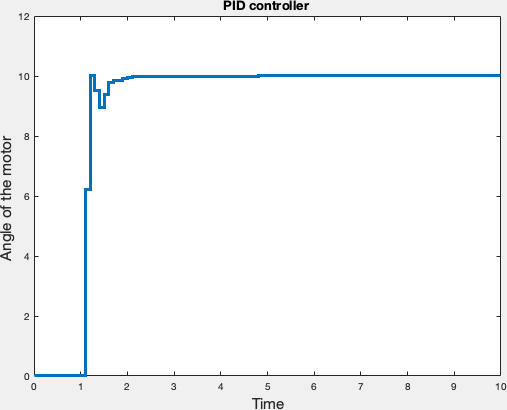
\includegraphics[width=\textwidth]{{sections/assets/pid_motor}
    \caption{PID controller for the LEGO EV3 motor to rotate 10 degrees}
    \label{fig1}
\end{figure}

\section{Conclusions}
For building a robot supposed to complete the task given in this project, the conclusion is that lego is not the best choice. Many of the lego parts are flexible and are connected to each other in a way that makes the robot very ``wobbly''. The accuracy of the robot arm was heavily reduced due to the flexibility of some lego parts. Also from section \ref{Results}, it can be seen that the fastest controller for the robot arm in terms of rise time and settling time was in fact the P controller for the vertical movement and the PD controller for horizontal movement. Despite this the included library functions from BrickPi3 for motor movement was used instead since the P and PD controllers made the robot ``wobble'' very much and there was risk of knocking the box of the industry platform. As mentioned the included library functions for motor movement was used instead since they achieved a good combination of being both quick and smooth.
For doing the task of taking a instruction from arrowhead, which was pick up the box or put down the box at different locations, our conclusion is that the robot could do it with some difficulties. The difficulties being that the lego flexibility reduced the accuracy of the robot arm which made the robot sometimes miss the box.

\section{Future improvements}
% Tackle the most obvious first
The result of this project can be improved in several ways: the most
obvious way is spending the necessary time to finalize all software
nodes and their interactions such that all milestones defined in
section~\ref{sec:milestones} are reached.

% Spend some time to ditch the additional hardware
The current robot system currently depends on some external hardware
which would be unnecessary if the Linux kernel was aware of all the
peripherals offered by the hardware. It may be worth it to investigate
why these are not already supported by NixOS and ultimately push the
eventual fixes upsteam. While improving the overall quality of this
project, it would also bump the overall quality of NixOS itself.

% An embedded system instead
An alternative to the current hardware setup and software stack would be
the design of a truly embedded system without a rich OS (Linux in this
case). A custom hardware design would allow the installation of multiple
sensors that could help in the problem space: such as a compass for
deriving the direction in which the robot is currently heading; and
directly designing the wideband-module of the DWM into the hardware, so
that the whole DWM-tag subsystem can be replaced. Further, an embedded
system would allow the implementation of a code-base that fully relies
on hardware interrupts\footnote{A feature more prominent and earier to
  work with on an embedded system, where a change in input voltage
  directly interrupts the processor (be it from a task of lower
  priority, or from sleep) to start a procedure to process data.} which
would enable the removal of any busy-while loops related to I/O. the
system would thus be made real-time capable if properly programmed. An
interrupt-oriented approach would allow the processor to sleep whenever
it has no data to process. This allows for a more responsive system, and
one that consumes less energy to operate.

% While not required, it would be more proper
Although the problem description does not call for a real-time system,
such an implementation would be much more proper for the problem domain,
and would more closely approximate how an actual industial system would
be implemented.

% Possible to apply formal analysis
Further, the implementation of such a system could be the subject for a
formal analysis with the lack of a rich OS that needlessly complicates
the call-stack.

% Can we port the current software stack?
The software-node based structure can readily be ported to a real-time
operating system (RTOS) if it allows the implementation of ``tasks''
that trigger on interrupts; and/or can be called from another task; and
if the RTOS implements message passing between these tasks. An example
for such a RTOS would be Real-Time Interrupt-driven Concurrency (RTIC)
\parencite{rtic}. Of possible interest would also be the MicroPython
project, which could allow minimal porting changes of the currently
available Python nodes if properly implemented for the target RTOS.
\parencite{micropython}.
%Robot hardware and lego
For the hardware side of the robot some other material than lego, like 3D printed body frames could be used to increase the physical stability of the robot itself. Also to make better or more advanced controllers for the robot arm motion, a dynamical model of the robot arm could be derived and put on state space representation since this is often advantageous if one wishes to make a good controller.



\appendix
\section{Team members}
The team's members are below listed (in no particular order) along with their areas of concern throughout the development of this project.
Emails are available on the title page of this document.

\begin{description}
\item[Viktor Sonesten] Repository maintainership; software packaging
  via Nix; data acquisition from the Decawave hardware; report
  typesetting; authorship of sections §1, §2.1, §2.4, §3, appendix B.

    \item[Lukas Karlsson]
    Embedded programming and
    Computer vision/position control.

    \item[Simon Sandberg]
    Position, grip control;
    sensory data integration, tuning; and
    embedded programming.

    \item[Oleksiy Mishchenko]
    Sensor implementation and tuning;
    implementation, tuning of control systems; and
    embedded programming.

    \item[Ruben Asplund]
    Arrowhead integration and embedded programming.
    Authorship of sections §1.4, §3.4 and the Arrowhead node in §3.3.

    \item[Ali Nouri]
    Embedded programming;
    inverse kinematics modeling; and
    navigation system design.

    \item[Ali Khademi]
    Dynamic equations and controller design for position.
\end{description}


\section{Work flow}
Every component of this project (code, documentation, models, simulations, etc.) is publicly hosted on GitHub at \href{https://github.com/tmplt/ed7039e}{https://github.com/tmplt/ed7039e}.

Using GitHub's auxiliary tools, each defined milestone is assigned to a GitHub repository project.
Each project contains a set of tasks that are marked as ``todo'', ``in progress'', or ``done''.
When all tasks in a project have been marked as ``done'', the milestone has been reached:
a feature has either been implemented, or a bug has been fixed, depending on the milestone definition.
For example, the milestone of implementing two-dimensional navigation is organized via the \href{https://github.com/tmplt/ed7039e/projects/1}{project under the same name}.

Once a week a meeting was held to wrap up the previous week and make any necessary preparations for the coming week:
such as assigning tasks, helping with any blocking issues, etc.

\subsection{Git work flow}
If one or more team members wishes to apply a change to the repository,
they create an appropriate branch in their fork of the repository,
commit their changes to this branch and create a pull request to the original repository.
After its submission it is up to the repository maintainer to verify that proposed changes are:
appropriate,
hold a certain quality (e.g., in the case of a code submission, that the code is sufficiently commented and understood),
and may be reproducibly built. % TODO: refer to the section on Nix?
If these criteria are not met, the required changes will be communicated to the pull request author(s) either via the GitHub's built-in review tools, or in person.
When the above criteria are met, the maintainer will merge the commits into the tree of the target branch.
The main branch of this project is denoted as the ``master'' branch wherein only working code should reside.
Any features that require an extensive implementation and/or testing period may reside in any amount of additional branches,
be it under the origin repository or under a fork.


% \section{System composition}
% The current plan is to build the robot mostly with the lego ev3 parts.\\ The mobile platform will be built with the parts present in the package given to the group in the beginning of the project. The arm, which will grip the cube, will be built from external lego parts and motors, the list of these parts will be submitted furing this Tuesday. A resberry pie will be used for the communication between sensors and motors, all calculations for the control systems will also be computed int it. A preliminary model has been calculated for the forward kinematics of the system, this will probably be updated and an inverse kinematic model will be derived. The decision has not yet been made on how the location of the robot will be calculatedl, some of the possible navigation systems that have been discussed are; LIDAR, using deckawave together with a sonar, using wifi triangulation and other solutions. 

\subsection{Structure of work}
\subsubsection{Milestones}
\subsubsection{Tecchnical solutions in the project}

\printbibliography

\end{document}
